\documentclass[twoside, single, authoryear, semicolon, 12pt]{lion-msc}
\usepackage{lipsum}
\usepackage{booktabs}
\usepackage{pifont}
\usepackage[version=4]{mhchem}
\usepackage{parskip}
\usepackage{float}

\title{Detecting Nitrogen Carriers in Planet-Forming Regions of Protoplanetary Disks}
\author{Niels de Klerk}

\major{Astronomy and Physics}
\affiliation{Leiden Observatory, Universiteit Leiden}

\newdate{date}{\day}{\month}{\year}           % definition of time and date using datetime package
% \newdate{date}{27}{08}{2010}
\date{\displaydate{date}}

\studentid{s3640477}                           % check you student ID, LaTeX does not do this
\abstract{Nitrogen is one of the most important elements for life on earth, and plays an important role in the chemistry of protoplanetary disks that are the birthplace for planets. However, the only nitrogen carrier detected in these disks is HCN. This thesis aims to investigate the detection of NO and NH\3 in the spectra taken by JWST MIRI MRS. For this, a grid of ProDiMo models with varying C and O abundances was used in combination with FLiTs to create spectra. The effects of the C and O abundances on the flux were investigated, and spectral regions of interest were selected. Furthermore, a new technique of detecting molecules using cross-correlation was studied. Utilizing this technique, molecules already detected in GWLup, Sz98, and V1094Sco were reaffirmed with a possible detection of NO in V1094Sco.}% limit your self to 1/2 page or 500 words
\dailysupervisor{Msc. Marissa Vlasblom \\ \hspace*{\fill}Msc. Aditya M. Arabhavi}
\supervisor{Prof. Dr. Ewine van Dishoeck \\ \hspace*{\fill}Prof. Dr. Inga Kamp} % Note that this should be a LION staff member!
\corrector{Dr. Matthieu Schaller}                      % This could be a LION staff member or your external supervisor

\degree{Bachelor of Science}                     % The default option is "Bachelor of Science", change if needed

\major{Astronomy and Physics}                  % The default option is "Physics", change if needed
%\major{Physics and Mathematics}

% optional cover picture - should be jpg or pdf
% \coverpicture{
\includegraphics[width=2cm]{Latex/lion-msc-logo.pdf}}

% Use this to make hyperlinks visible in the document.
\hypersetup{colorlinks=true}

% ---------------------------------------------------------------- My defintions!
% \renewcommand{\vec}[1] {\ensuremath{ \overrightarrow{ #1 } }}
\renewcommand{\vec}[1] {\ensuremath{ \mathbf{ #1 } }}
% \bra \ket \braket and \proj
\newcommand{\bra}[1]{\ensuremath{\langle #1 \vert}}
\newcommand{\ket}[1]{\ensuremath{\vert #1 \rangle}}
\newcommand{\braket}[2]{\ensuremath{\langle #1 \vert #2 \rangle}}
\newcommand{\proj}[1]{\ensuremath{\vert #1 \rangle \langle #1 \vert}}

\newcommand{\kpar}{\ensuremath{k_\parallel}}

\newcommand{\4}{$_4$}
\newcommand{\3}{$_3$}
\newcommand{\2}{$_2$}
% ----------------------------------------------------------------

% \usepackage{tocloft}
% \renewcommand{\cftchapdotsep}{\cftdotsep}
\begin{document}

% roman numbering in the table of contents section
\pagenumbering{roman}

\maketitle

% Table of contents:  it is a good idea to include this into your thesis
\tableofcontents
\cleardoublepage
\pagenumbering{arabic}
\chapter{Introduction}
The nebular hypothesis was first proposed in \textit{The Principia} by Emanuel Swedenborg in 1745. Immanuel Kant developed the theory further in 1752 and later modified by Pierre-Simon Laplace in 1796. The theory states that a planetary system is formed from a slowly rotating gas cloud that collapses into a disk. Centuries later, the first protoplanetary disk was observed by O'Dell using the Hubble Space Telescope \citep{ODell1993}. In recent years, the Atacama Large Millimeter/submillimeter Array (ALMA) has imaged a large collection of these protoplanetary disks, showing a wide variety of structures and compositions (e.g. \cite{gardner2025exoalmaxialmaobservations, shoshi2025alma2dsuperresolutionimaging}). The JWST MIRI mid-INfrared Disk Survey (MINDS) team uses the JWST to investigate the inner parts of protoplanetary disks (e.g. \cite{Arabhavi_2025, Vlasblom_2025}). The study of protoplanetary disks is important to find answers to the fundamental questions, 'How did life arise?' and 'Are we alone in the universe?'.

The spectrum of protoplanetary disks can tell us a lot about the properties of the disk and the host star. An important example is an observation of the disk around a T Tauri star Sz98 \citep{Gasman_2023}. Using MIRI on the JWST, they probed the inner regions of the disk. They detected CO$_2$, H$_2$O, OH, CO, and HCN. Furthermore, no other organics were detected, suggesting a low C/O ($<$0.5) ratio. This result differed from the ratio found using ALMA ($>$1), which probed the outer regions. This highlights the complexity of disks and their chemistry.

However, this observation is not necessarily representative of disks. \cite{colmenares2024jwstmiridetectioncarbonrichchemistry} observed a disk around the T Tauri star DoAr 33 with an exceptionally high C/O ratio of 2-4. In addition to CO, H\2O, and CO\2, like in the Sz98 disk, the more complex carbohydrates C\2H\2 and C\4H\2 were found. The presence of these molecules is indicative of this high ratio. A possible explanation for this carbon-rich environment is the slow accretion rate of the star, which results in slowing the radial mixing and the persistence of the carbon-grain destruction.

Observations of the protoplanetary disk around the T Tauri star GW Lup have given the first detection of $^{13}$CO$_2$ in a protoplanetary disk. \cite{Grant_2023} The combination with the spectral resolution of the JWST-MIRI and the high SNR allows for the detection of weaker spectral features. Notably, the deduced N$_{CO_2}$/N$_{H_2O}$ was significantly higher than previously thought. This could indicate a cavity between the H$_2$O and CO$_2$ snowlines. These findings show the new possibilities JWST provides for studying disk structures. 

% The effects of a cavity on the spectrum were studied by \cite{vlasblom2023midinfraredspectrattauri}. It was speculated that 'CO$_2$-only sources' have inner cavities which extend beyond the H$_2$O snowline, but stay within the CO$_2$ snowline. By running thermo-chemical models with different inner cavity sizes, it was shown that N$_{CO_2}$/N$_{H_2O}$ grows as the size of the cavity grows and then sharply drops. The conclusions drawn from this can help to interpret the spectra of disks.


\section{Formation and Evolution of Disks}
Molecular clouds are large collections of gas and dust. When these clouds are perturbed, parts of the cloud can become dense enough, making them collapse under their own gravity. This will result in the creation of a star surrounded by gas and dust. The angular momentum of each of the particles is randomly oriented, but on average, the angular momentum vector is pointed in a certain direction. Two particles colliding will cause them to exchange angular momentum. If many collisions happen, all the angular momenta other than the average angular momentum vector get canceled out. This results in the formation of a disk around the pre-main-sequence star.
The evolution of the disk can be categorized into 4 classes \citep{1987ApJ...312..788A}. Class 0 objects are objects where an optically thick envelope surrounds the protostar. Class I objects have a star and disk but are still embedded in an optically thick envelope. The star and disk become visible in class II objects as the star has become bright enough to blow away the envelope. In class III objects, the disk has largely been depleted of gas and dust, leaving behind planets and planetesimals. 
% % Factors that influence the evolution



% The protoplanetary disk has structure, namely the radial structure and the vertical structure. The innermost regions ($<$10 AU) of the disk are the hottest and receive the most radiation. Most of the molecules are in gaseous form in this region, except for some silicates and metals. The star heavily influences the chemistry. The intermediate regions (10-100 AU) have lower temperatures, allowing molecules like water to condense. The outer regions ($>$100 AU) are the coldest in the disk. Molecules have formed ice here, making them inert. \\
% The height of the disk is also an important factor in its structure. The midplane is the horizontal plane through the center of the disk. Most dust particles settle around the midplane, whereas the gas particles are further out. The midplane is also colder than the outside of the disk as it receives less light from the star. The protoplanetary disk tends to flare outwards. Close to the star, the disk is fairly compact, but when you go outwards from the star, the disk gets more and more extended from the midplane. 

% \begin{figure}[H]
%     \centering
%     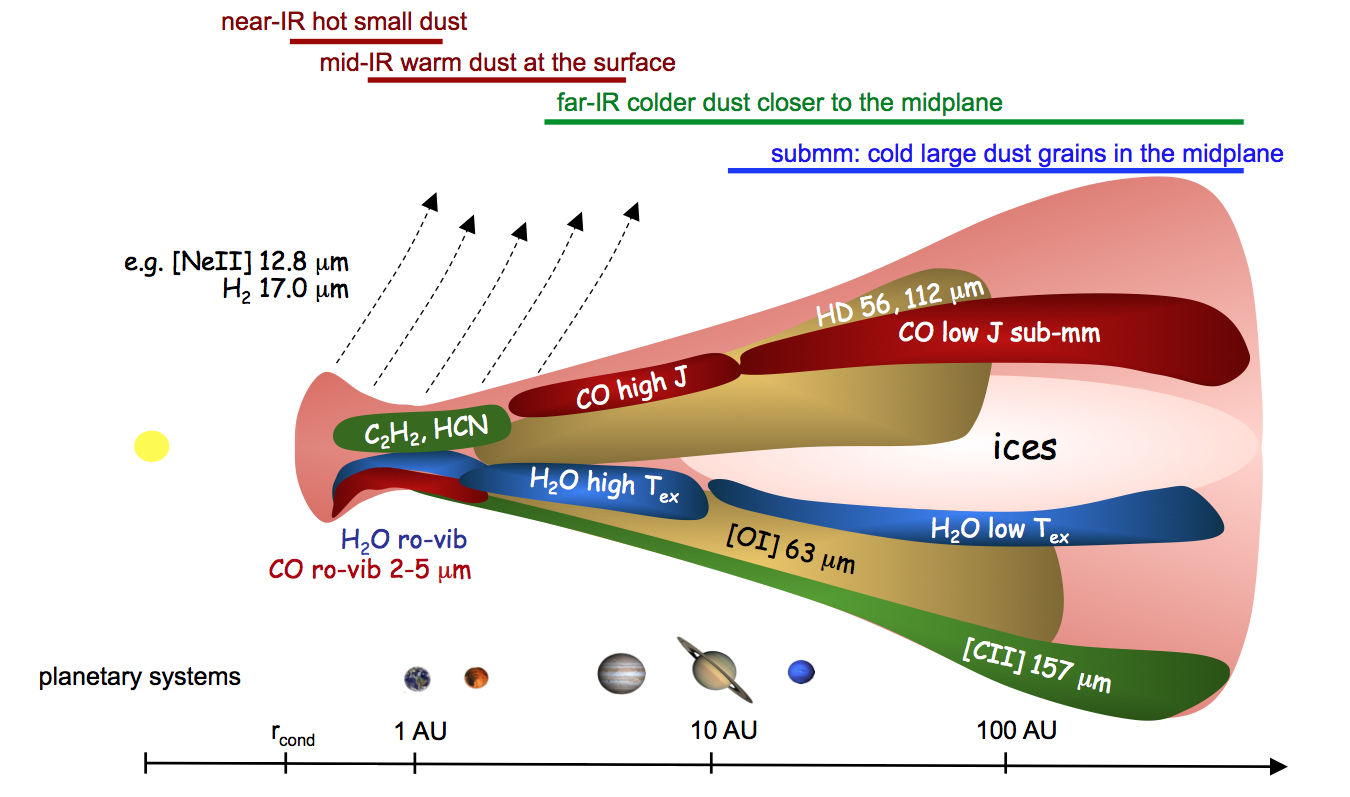
\includegraphics[width=\linewidth]{Figures/disk-sketch.png}
%     \caption{A schematic representation of a protoplanetary disk. The planets in the solar system are shown as a point of reference. \cite{inproceedings}}
%     \label{fig: enter-label}
% \end{figure}

\section{Disk Chemistry}
Explaining something about general chemistry, including in-depth nitrogen chemistry

discuss \cite{van_Gelder_2024}
\section{Emission Mechanisms}
It is important to understand how molecules emit photons. In this section, we will explain how these processes work. This is largely based on Chapter 11 of \cite{1979rpa..book.....R}. 

When a molecule transitions from a higher energy state to a lower energy state, it emits a photon with a wavelength

\begin{equation}
    \lambda=\frac{hc}{\Delta E}
\end{equation}

where $\Delta E$ is the difference in energy between the two states. Molecules order themselves in different energy states following the rules of thermodynamics. In thermal equilibrium, they organize according to the Boltzmann distribution (\autoref{eq: boltzmann}). 

\begin{equation}
    \frac{N_i}{N}=\frac{g_i\exp{(-E_i/k_BT)}}{Z}
    \label{eq: boltzmann}
\end{equation}

with $N_i$ the number of molecules in state $i$, $E_i$ the energy of state $i$, $g_i$ the degeneracy of that energy state, $T$ the temperature of the molecule and $Z$ the partition function $Z=\sum_j g_j\exp{(-E_j/k_BT)}$.
Different transitions can take place within molecules. This section will discuss the 3 most fundamental transitions: electronic, vibrational, and rotational.

\subsection{Electronic Transition}
The transition of the highest energy is the electronic transition. In this transition, an electron jumps from an orbital with higher energy to one with lower energy. For simplicity, we will examine the hydrogen atom. The energy levels in the hydrogen atom are determined by 

\begin{equation}
    E^e=-\frac{13.6\mathrm{ eV}}{n^2},
    \label{eq: electronic}
\end{equation}
where n is the principal quantum number. The energy 13.6 eV in \autoref{eq: electronic} is called the ionization energy. This is the energy of an electron in the ground state needs to be gained to get unbound, resulting in the ionization of the atom. The transitions to $n=1$ are called the Lyman series (Ly$\alpha$, Ly$\beta$, etc.). The Balmer series corresponds with the transitions to $n=2$ (H$\alpha$, H$\beta$, etc) and the Paschen series with $n=3$. The degeneracy of each state is $g(n)=2n^2$. The energy levels and the line strengths corresponding to transitions between these energy levels are shown in \autoref{fig: elec}.

\begin{figure}[H]
    \centering
    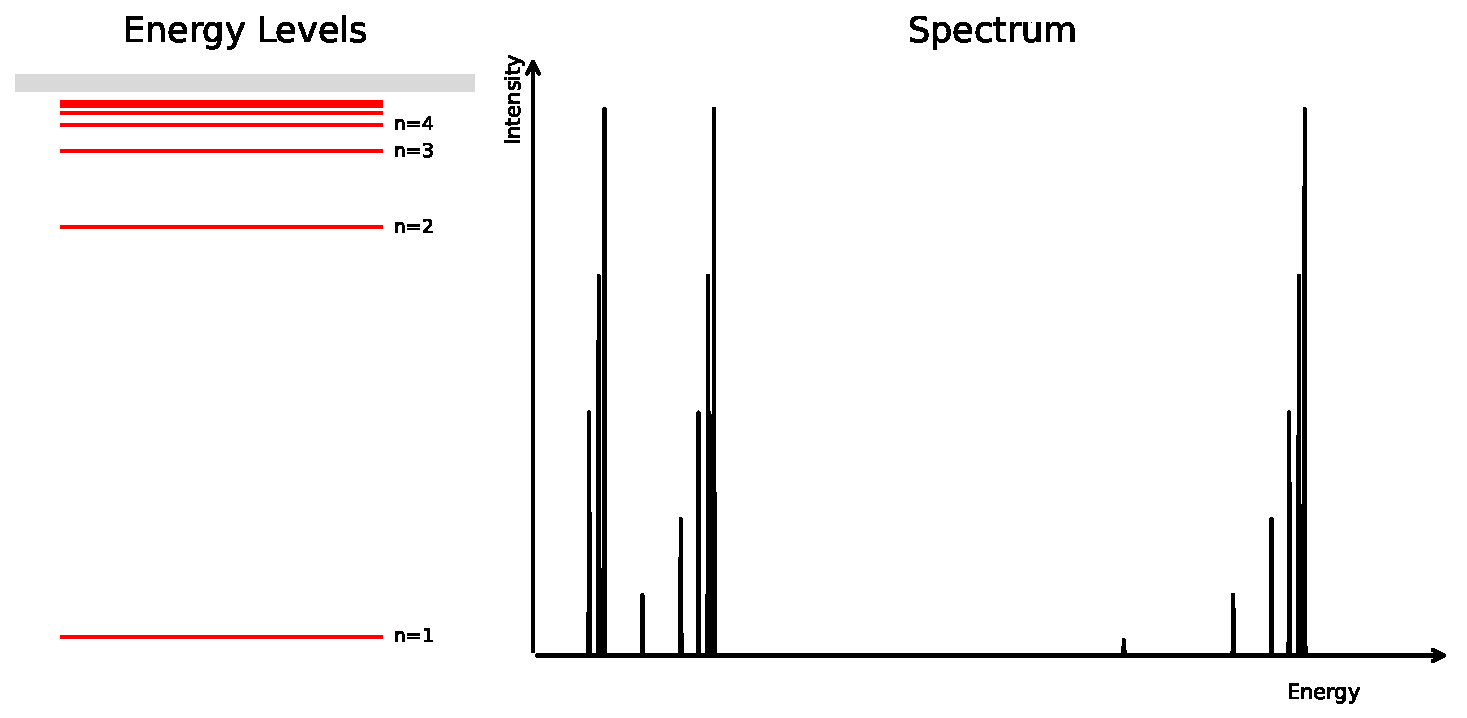
\includegraphics[width=\linewidth]{Figures/ElecSpectrum.pdf}
    \caption{The electronic energy levels and the corresponding spectrum, where the molecules follow the Boltzmann distribution}
    \label{fig: elec}
\end{figure}

The electronic transitions typically occur in the ultraviolet (UV) and visible (VIS) parts of the electromagnetic spectrum. For example, the transition from n=2 to n=1, the Ly$\alpha$ transition, occurs at 121.567 nm.


\subsection{Vibrational Transition}
Vibrational transitions \textbf{how do i start this sentence}. This changes the vibration of the molecule. The bonds between atoms in a molecule can be viewed as springs connecting the atoms. These springs can have different motions, such as stretching and bending. 

\begin{equation}
    E^{vib}=\hbar\omega(v+1/2)
\end{equation}

with $\hbar$ the reduced Planck constant, $\omega=\sqrt{\frac{k}{\mu}}$ with $k$ the force constant and $\mu$ reduced mass, and $v$ the vibrational quantum number. Transitions between energy states follow the selection rule: $\Delta v=\pm 1$. This means the only permitted transitions occur between energy levels with a vibrational quantum number that is one lower or higher than the current state. This results in the difference in energy between states to be

\begin{equation}
    \Delta E^{vib}=\hbar\omega.
\end{equation}

 Plotting the energy levels and the resulting spectrum gives \autoref{fig: vib}.

\begin{figure}[H]
    \centering
    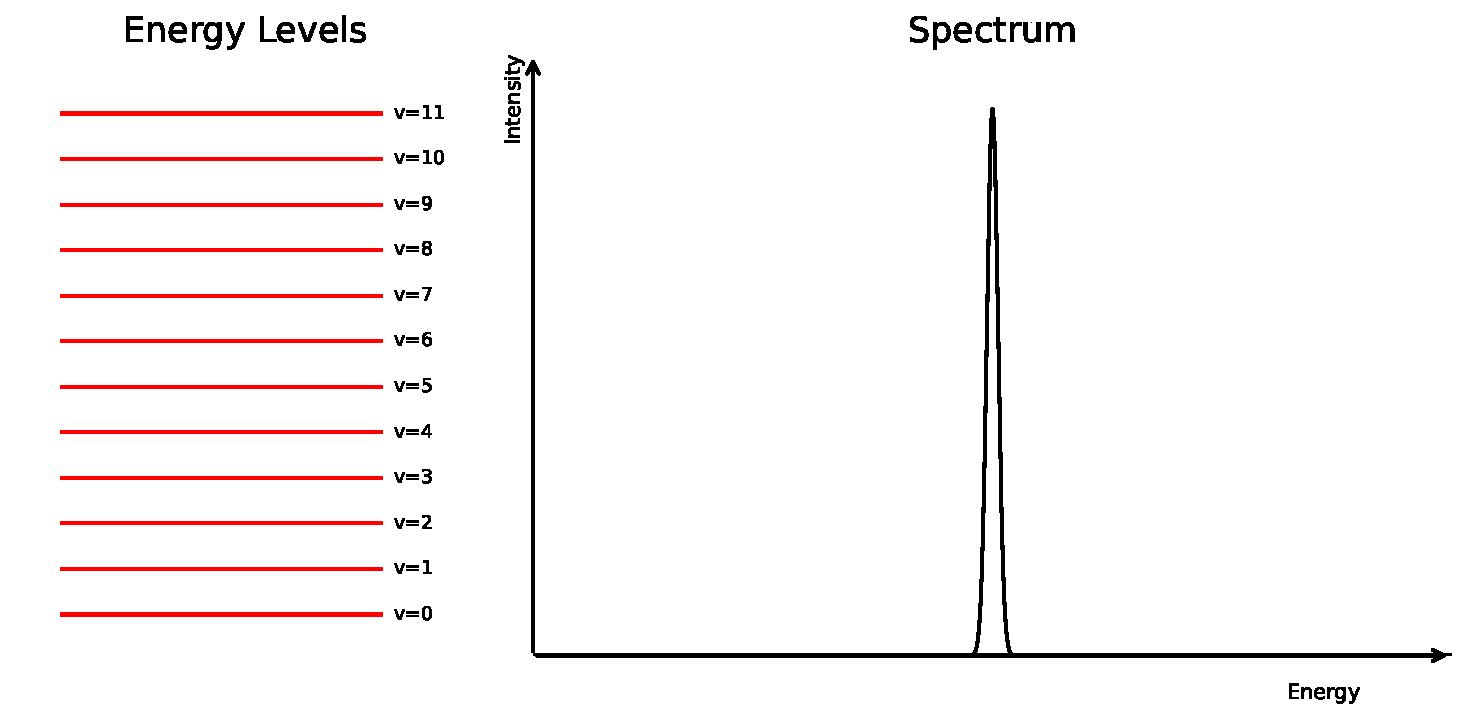
\includegraphics[width=\linewidth]{Figures/VibSpectrum.pdf}
    \caption{The vibrational energy levels and the corresponding spectrum}
    \label{fig: vib}
\end{figure}

The vibrational transitions typically occur in the infrared (IR) part of the electromagnetic spectrum. 


\subsection{Rotational Transition}
The transition with the lowest energy is the rotational transition. This transition changes the angular momentum of the molecule. 

\begin{equation}
    E^{rot}=B_eJ(J+1)
\end{equation}

where J is the rotational quantum number

\begin{equation}
    \Delta  E^{rot}=2B_e(J+1)
\end{equation}

The degeneracy of each state is $g(n)=2J+1$. Transitions between energy states follow the selection rule: $\Delta J=\pm 1$. This means the only permitted transitions occur between energy levels with a rotational quantum number that is one lower or higher than the current state. Plotting the energy levels and the resulting spectrum following the Boltzmann distribution gives \autoref{fig: ro}.

\begin{figure}[H]
    \centering
    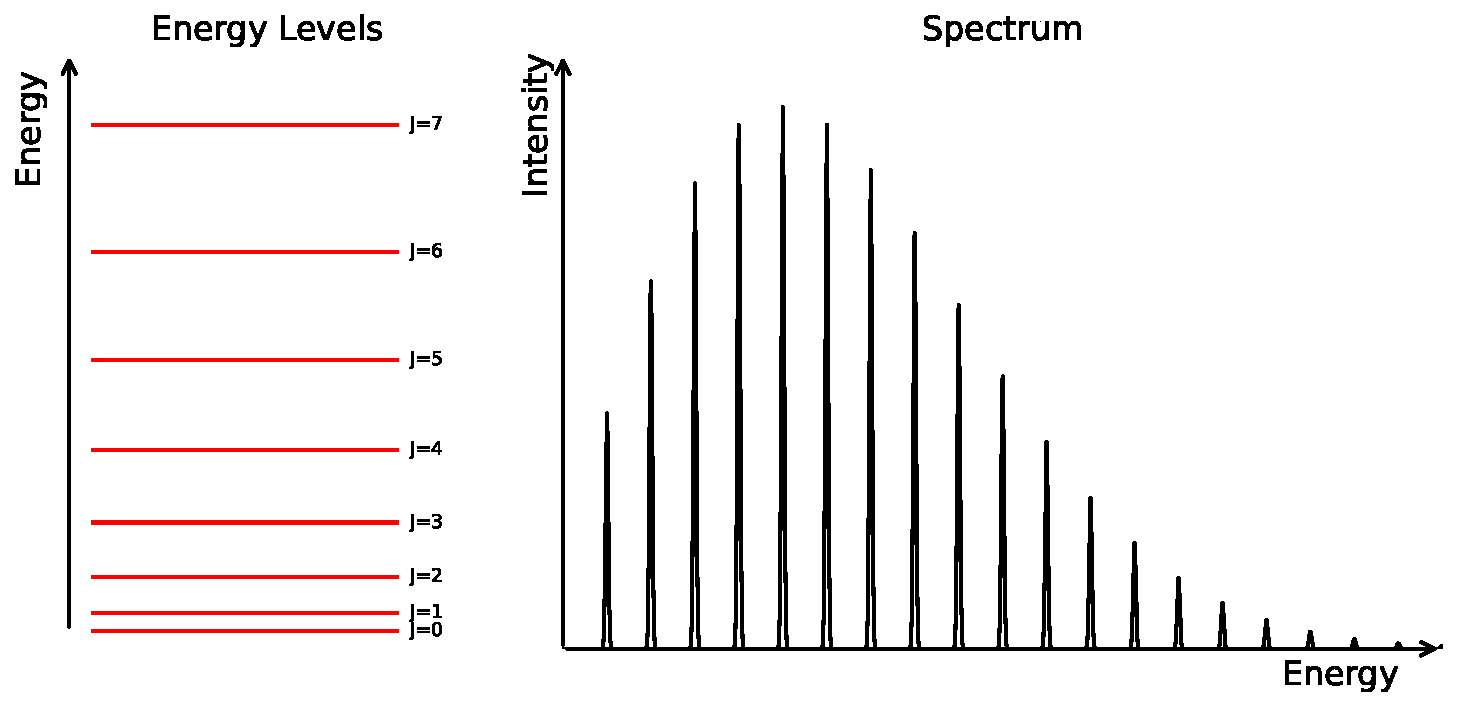
\includegraphics[width=\linewidth]{Figures/RoSpectrum.pdf}
    \caption{The rotational energy levels and the corresponding spectrum, where the molecules follow the Boltzmann distribution}
    \label{fig: ro}
\end{figure}

The electronic transitions typically occur in the microwave and radio parts of the electromagnetic spectrum.

\subsection{Ro-vibrational Transition}
In nature, pure vibrational transitions are rare. More often than not, the vibrational transitions are accompanied by rotational transitions. The combination of these two transitions is called a ro-vibrational transition. Transitions between energy states follow the selection rules: $\Delta v=\pm 1$, $\Delta J=0, \pm 1$. Plotting the energy levels and the resulting spectrum following the Boltzmann distribution gives \autoref{fig: rovib}.

\begin{figure}[H]
    \centering
    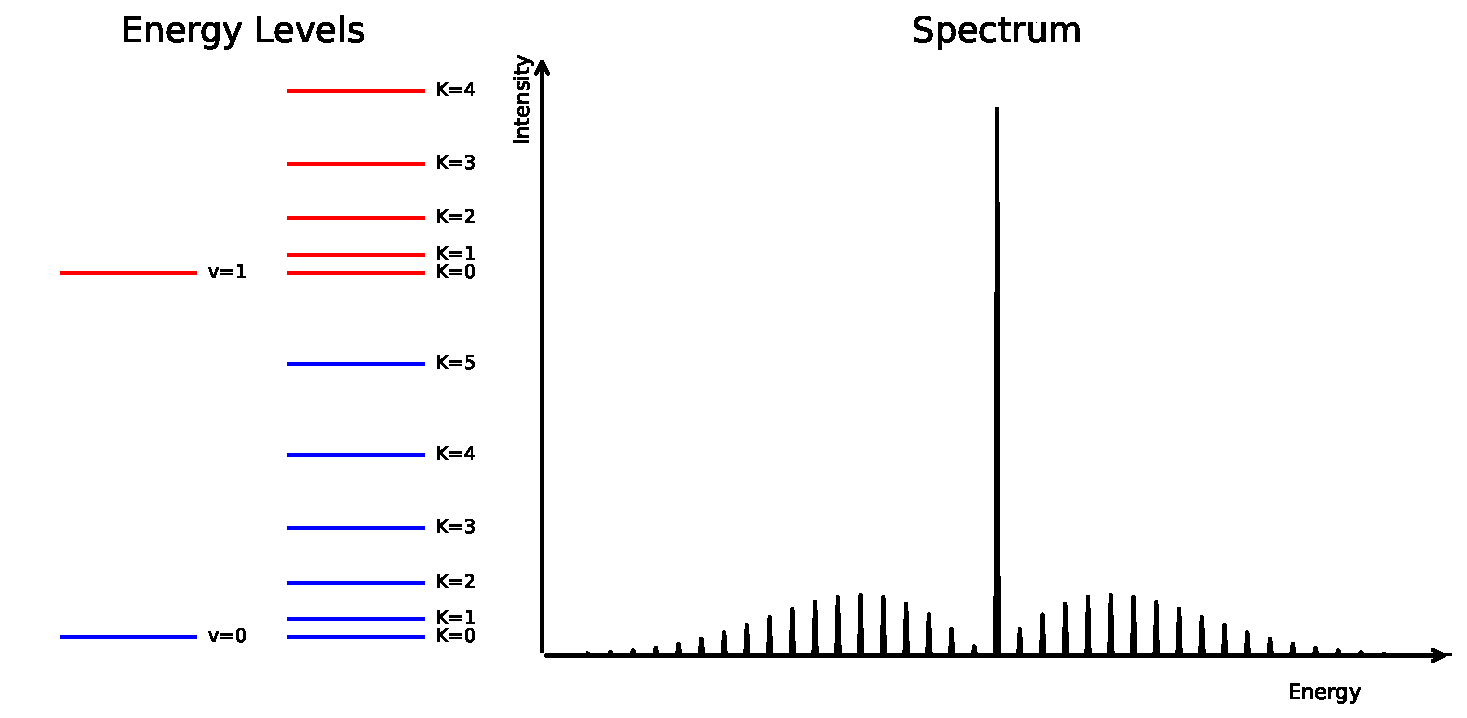
\includegraphics[width=\linewidth]{Figures/RoVibSpectrum.pdf}
    \caption{The ro-vibrational energy levels and the corresponding spectrum, where the molecules follow the Boltzmann distribution}
    \label{fig: rovib}
\end{figure}

In \autoref{fig: rovib}, a distinctive shape is visible: P, Q, and R branches. The P branch is the set of peaks with a lower energy than the central peak. The Q branch is the central peak, and the set of peaks on the higher energy side of the peak is the R branch. The P, Q, and R branches correspond to $\Delta J=1, 0, -1$ respectively. For some molecules and some vibrational modes, the transition with $\Delta J=0$ is forbidden. This also means that the Q branch is missing in the spectrum.

\section{JWST MIRI MRS}
The James Webb Space Telescope (JWST) was launched on the 25th of December 2021. This new telescope was a big leap forward for space research. One of the instruments on board is the Mid-Infrared Instrument (MIRI). This instrument is used for observation in the mid-infrared, as the name suggests. 

\section{Modeling of Protoplanetary Disks}
Some of the properties of the protoplanetary disks can be directly inferred from disk measurements. For instances where this is not the case, we would still like to learn more from our data via a different method. We can use models to simulate the protoplanetary disk and generate synthetic data to compare to actual observations. There are various types of models. Ranging from 0D slab models to thermo-chemical disk models. 
\textbf{EXPLAIN WHAT FIDUCIAL IS}
\subsection{ProDiMo}
For our research, we run simulations using the PROtoplanetary Disk Model (ProDiMo), a thermo-chemical disk model.
\subsection{FLiTs}
The output of those simulations is then put through Fast Line Tracing system (FLiTs) to get an accurate spectrum of the disk. 

\section{Research Objectives and Scope}
First, we want to investigate how nitrogen carriers depend on the abundances of carbon and oxygen. Furthermore, we aim to investigate how the emission of nitrogen carriers changes after increasing the nitrogen abundance. Next, we want to develop a method to detect nitric oxide (NO) and ammonia (NH\3) in the spectra of protoplanetary disks using JWST MIRI MRS. 
We present the methodology in \autoref{Ch: Methods}. The data and results are shown in \autoref{Ch: Results}. We discuss the results and their implications in \autoref{Ch: Discussion}. In \autoref{Ch: Conclusion}, we conclude our thesis.


\chapter{Methods}\label{Ch: Methods}
\section{ProDiMo Simulations}

\begin{table}[!ht]
\centering
\begin{tabular}{@{}lll@{}}
                                  &                             &                            \\ \hline\midrule
\textbf{Property}                 & \textbf{Symbol}             & \textbf{Value}             \\ \midrule
Stellar mass                      & M$_\ast$                    & 0.7M$_\odot$               \\
Effective Temperature             & T$_\ast$                    & 4000 K                     \\
Stellar Luminosity                & L$_\ast$                    & 1 L$_\odot$                \\
UV excess                         & f$_{UV}$                    & 0.01                       \\
UV powerlaw index                 & p$_{UV}$                    & 1.3                        \\
X-ray luminosity                  & L$_x$                       & 10$^{30}$ erg/s              \\
X-ray emission temperature        & T$_x$                       & 2$\times10^7$ K            \\ \midrule
Strength of interstellar UV       & $\chi^{ISM}$                & 1                          \\
Strength of interstellar IR       & $\chi^{ISM}_{IR}$           & 0                          \\
Cosmic ray H$_2$ ionization rate  & $\zeta_{CR}$                & $1.7\times10^{-17} s^{-1}$ \\ \midrule
Inner disk radius                 & R$_{in}$                    & 0.05 au                    \\
Outer disk radius                 & R$_{tap}$                   & 30 au                      \\
Column density power index        & $\epsilon$                  & 1                          \\
Reference scale height            & H$_g$ (100 au)              & 10 au                      \\
Flaring power index               & $\beta$                     & 1.15                       \\ \midrule
Minimum dust particle radius      & a$_{min}$                   & 0.05 $\mu$m                \\
Maximum dust particle radius      & a$_{max}$                   & 3000 $\mu$m                \\
Dust size dist. power index       & a$_{pow}$                   & 3.5                        \\
Turbulent mixing parameter        & $\alpha_{settle}$           & 0.001                      \\
Refractory dust composition       & Mg$_{0.7}$Fe$_{0.3}$SiO\3 & 60 \%                      \\
                                  & amorph. C                   & 15 \%                      \\
                                  & porosity                    & 25 \%                      \\
PAH abundance rel. to ISM         & f$_{PAH}$                   & 0.01                       \\
Chemical heating efficiency       & $\gamma^{chem}$             & 0.2                        \\ \midrule
Distance to the observer          & d                           & 140 pc                     \\ \bottomrule
\end{tabular}
\caption{Disk parameters used for the grid of ProDiMo models}
\label{tab: parameters}
\end{table}

To investigate whether we can detect NO and NH\3 in the spectra of protoplanetary disks and how nitrogen carriers depend on the C and O abundance, we used a grid of ProDiMo models with varying abundances of C and O. The parameters with which the models were run are given in \autoref{tab: parameters}.

\begin{equation}
    \epsilon_X\equiv\log\frac{N_X}{N_H}+12
\label{eq: abundance}
\end{equation}

The abundances are defined as in \autoref{eq: abundance}, where the abundance ($\epsilon_X$) depends on the natural log of the ratio of the number density of that element X ($N_X$) to the number density of hydrogen ($N_H$). In this system, $\epsilon_H=12$ by definition. The differences in abundances of C and O compared to solar abundances were varied between -0.5 and 0.5 in steps of 0.25, where a difference of 0 corresponds to the solar abundance. The grid contains 25 models, with the fiducial model in the middle, which is based on the solar abundances of C and O (see \autoref{tab: abundances}). Furthermore, we increased the nitrogen abundance by an order of magnitude compared to the solar abundance to see what the effects on the spectrum are and to enhance the spectral features of nitrogen carriers.

\begin{table}[!ht]
\centering
\begin{tabular}{@{}ccc@{}}
                                  &                             &                            \\ \hline\midrule
\textbf{Element} & \textbf{+12 Abundance} & \textbf{Variation}            \\ \midrule
H                & 12                     & Fixed                         \\
He               & 10.98                 & Fixed                         \\
C                & 8.14                  & {[}-0.5, -0.25, 0, +0.25, +0.5{]} \\
N                & 8.90                  & Fixed                         \\
O                & 8.48                  & {[}-0.5, -0.25, 0, +0.25, +0.5{]} \\
Ne               & 7.95                  & Fixed                         \\
Na               & 3.36                  & Fixed                         \\
Mg               & 4.03                  & Fixed                         \\
Si               & 4.24                  & Fixed                         \\
S                & 5.27                  & Fixed                         \\
Ar               & 6.08                  & Fixed                         \\
Fe               & 3.24                  & Fixed                         \\
PAH              & 3.44                  & Fixed                         \\ \bottomrule
\end{tabular}
\caption{The elemental abundances used in the simulation of the grid of ProDiMo models}
\label{tab: abundances}
\end{table}



The output of the ProDiMo model grid was used to generate the mid-infrared spectra using FLiTs. The full spectrum includes emission from C\2H\2, CH\4, CO, CO\2, H\2O, HCN, NH\3, NO, OH. In addition, FLiTs produced the spectra containing the emissions of the individual molecules. The FLiTs spectra were calculated at a very high spectral resolution ($R=1\cdot10^5$). To make the spectra more comparable to the JWST MIRI MRS spectra, we convolved the spectrum to a resolving power of $R = \lambda/\Delta\lambda = 3000$ using a Gaussian kernel to create a spectrum of the correct resolving power. The value of 3000 was chosen as it is approximately the average resolving power of the JWST MIRI MRS \citep{Argyriou_2023}. 

Noise was added to the simulated spectra to make them as realistic as possible. The observations obtained by the MINDS JWST GTO program have a signal-to-noise ratio (SNR) of 300 \citep{henning2024mindsjwstmirimidinfrared}.  To make the simulated data align with an $SNR = 300$, the minimum of the simulated spectrum before continuum subtraction was used to find the variance $\sigma^2$ by using \autoref{eq: SNR}.
\begin{equation}
    SNR = \frac{F_{min}}{\sigma}\Rightarrow\sigma=\frac{F_{min}}{SNR}
    \label{eq: SNR}
\end{equation}
The variance $\sigma^2$ was then used to add Gaussian noise to each flux value following \autoref{eq: noise}.
\begin{equation}
    \tilde{F}_i = F_i + \varepsilon_i,\;\varepsilon_i\sim\mathcal{N}(0, \sigma^2)
    \label{eq: noise}
\end{equation}
After applying this noise, we subtracted the continuum to get the spectrum. This spectrum was subsequently used to analyze the different molecules that compose it.


The flux density provided by FLiTs is in units of Jansky. To obtain the flux, we integrated the flux density by first converting the flux density from per unit frequency to per unit wavelength using \autoref{eq: conversion}.

\begin{equation}
    F_\lambda=\frac{c}{\lambda^2}F_\nu
    \label{eq: conversion}
\end{equation}

Different species emit light in distinct spectral regions. To classify these regions, we split the entire spectrum into windows of 0.001 $\mu$m from 4.9 to 27.5 $\mu$m. Next, we integrate the spectrum for each species in that window and note the species that has the highest flux in that region. Doing this for all models and taking the mode gives the species for each window that has the strongest emission for most of the simulated spectra.  


\section{Cross-Correlation Technique}
For our analysis, we used cross-correlation. This is a signal detection technique used to detect weak signals. We implemented this to detect the weak spectral features of NO and NH\3. It is defined as follows. 

\begin{equation}
    R_{fg}(\tau)=\int^\infty_{-\infty}\overline{f(t)}g(t+\tau)dt
\end{equation}

where $R_{fg}(\tau)$ is the cross-correlation, $f$ and $g$ are functions, and $\tau$ is the lag. As all our functions are real valued, we can omit the complex conjugation in the integrand.
% The autocorrelation is the cross-correlation of a function with itself

% \begin{equation}
%     R_{ff}(\tau)=\int^\infty_{-\infty}\overline{f(t)}f(t+\tau)dt
% \end{equation}

\begin{figure}[H]
    \centering
    \includegraphics[width=0.5\linewidth]{VISUALIZE CROSSCORRELATION}
    \caption{Caption}
    \label{fig:enter-label}
\end{figure}

To test the spectra for the presence of specific molecules, we used the emissions for each species across the model grid. The emissions per molecule for each model were added together and divided by the maximum to normalize them. We used this template emission to cross-correlate with the spectrum containing all the species. The cross-correlation should peak when the template spectrum matches the spectrum containing all the species. To quantify the height of the peak, we calculated the difference between the height of the peak and the median value of the cross-correlation in a small region around the peak. We took the median as this is less susceptible to outliers to capture the general trend around the peak more optimally. We used hypothesis testing to test whether or not there is statistical evidence to say the molecule is present. We had the following null hypothesis and alternative hypothesis

\begin{equation}
    H_0: \text{The height of the peak in the cross-correlation is caused by noise}
\end{equation}
\begin{equation}
    H_1: \text{The height of the peak in the cross-correlation is caused by the molecule}
\end{equation}

To assess the significance of the peak in cross-correlation, we used a Monte Carlo simulation to simulate 10000 synthetic spectra under the null hypothesis. First, we take all the flux values we have for different wavelength values. Second, we sample with replacement from the flux values until we have a collection of values that is the same size as the original set. Third, we take the cross-correlation and calculate the difference between the height of the peak and the median value of the cross-correlation in a small region around the peak. The value of the test statistic is deemed significant when it exceeds 95\% of the values from the simulated data ($\alpha=0.05$)


\section{Observations}
After looking at the simulated spectra, we wanted to apply our techniques to observations made with JWST MIRI MRS. We have access to 3 sources  GWLup \citep{Gasman_2023}, Sz98 \citep{Grant_2023}, and V1094Sco \citep{taboneinprepp}. The spectra we received were already continuum-subtracted and are shown in \autoref{fig: Measurements}. However, the continuum subtraction left artifacts in the spectrum. \cite{Grant_2023} has listed the regions in the spectrum containing such artifacts, and we used their list of regions to mask out the artefacts. Furthermore, we utilized LTE models to fit the observed spectra. This was used to find the emission of specific molecules and subtract them from the spectrum. This was used to find weaker emissions of other molecules in the residuals. 
\textbf{MORE EXPLANATION NEEDED}

\begin{figure}[H]
    \centering
    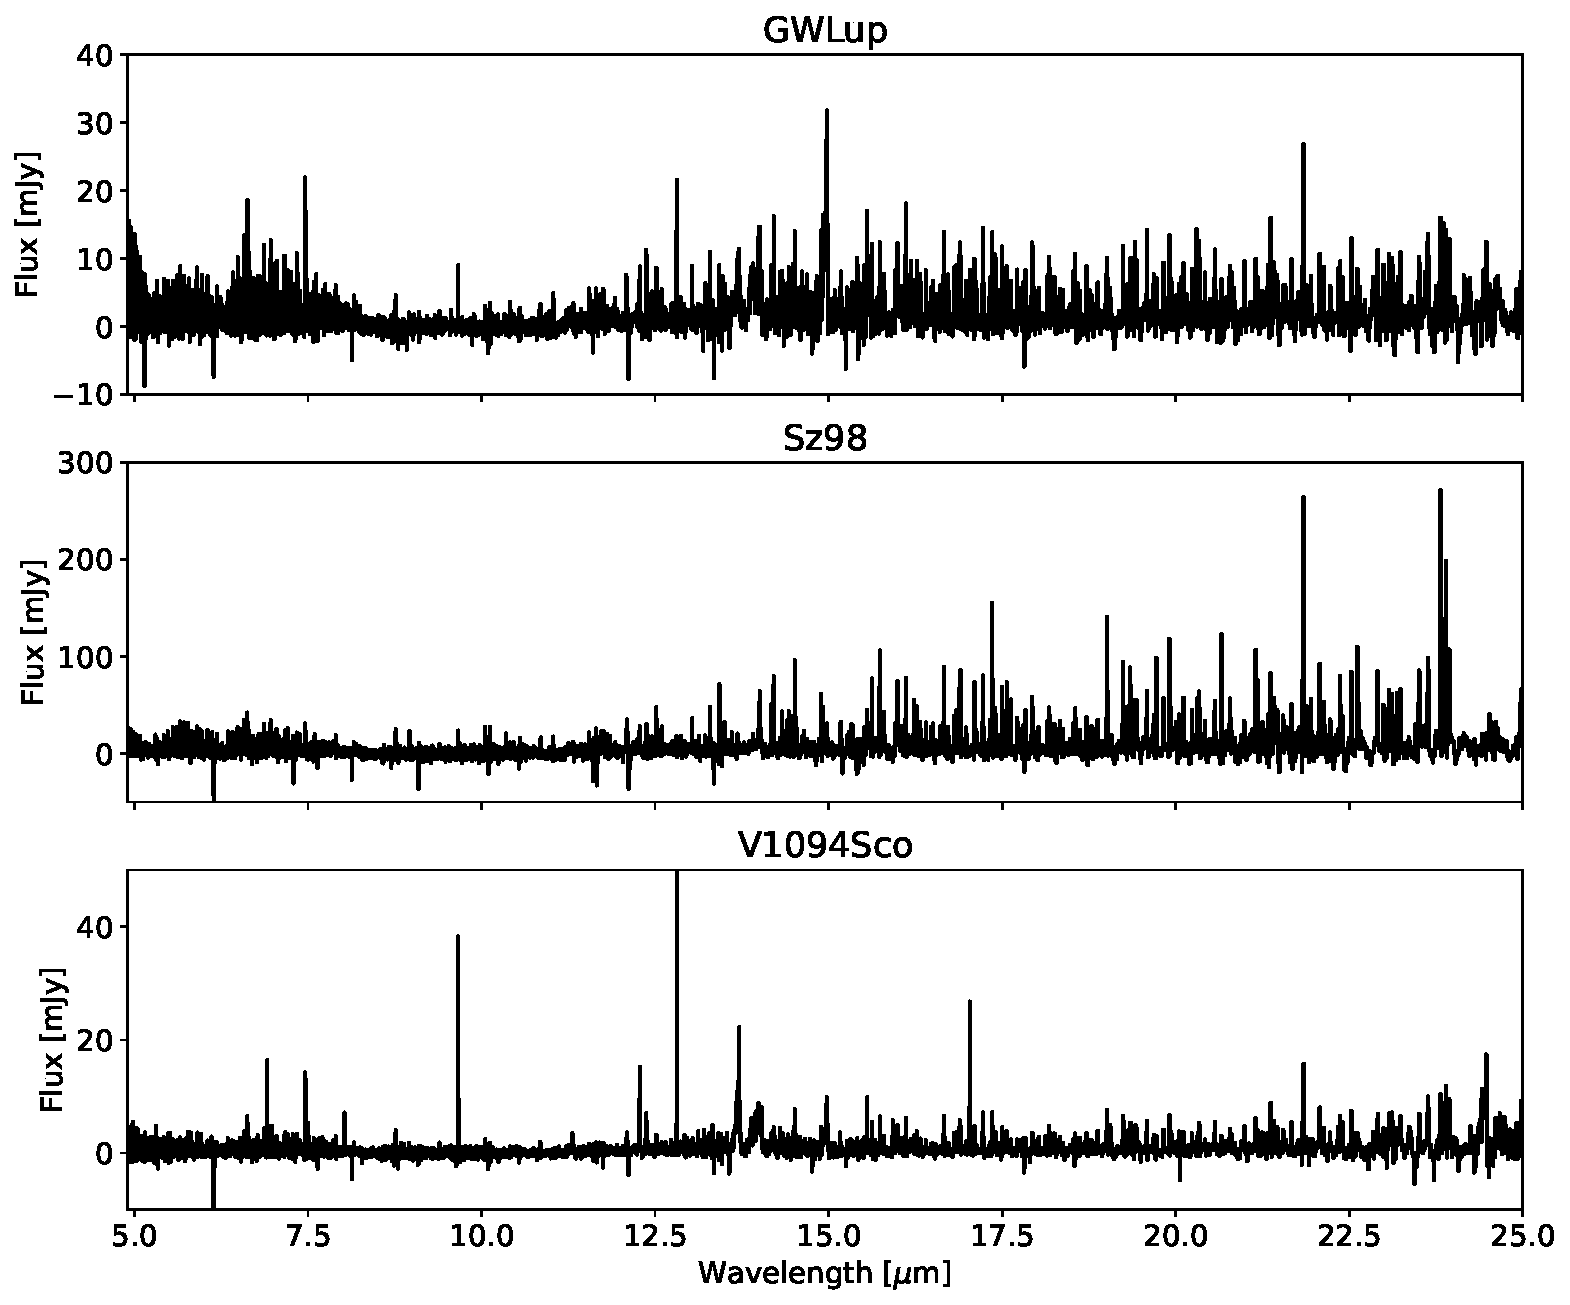
\includegraphics[width=\linewidth]{Figures/Measurements.pdf}
    \caption{The continuum subtracted spectra of GWLup \citep{Gasman_2023}, Sz98 \citep{Grant_2023}, and V1094Sco \citep{taboneinprepp}}
    \label{fig: Measurements}
\end{figure}



\chapter{Results}\label{Ch: Results}
\section{ProDiMo Output}
\begin{figure}[H]
    \centering
    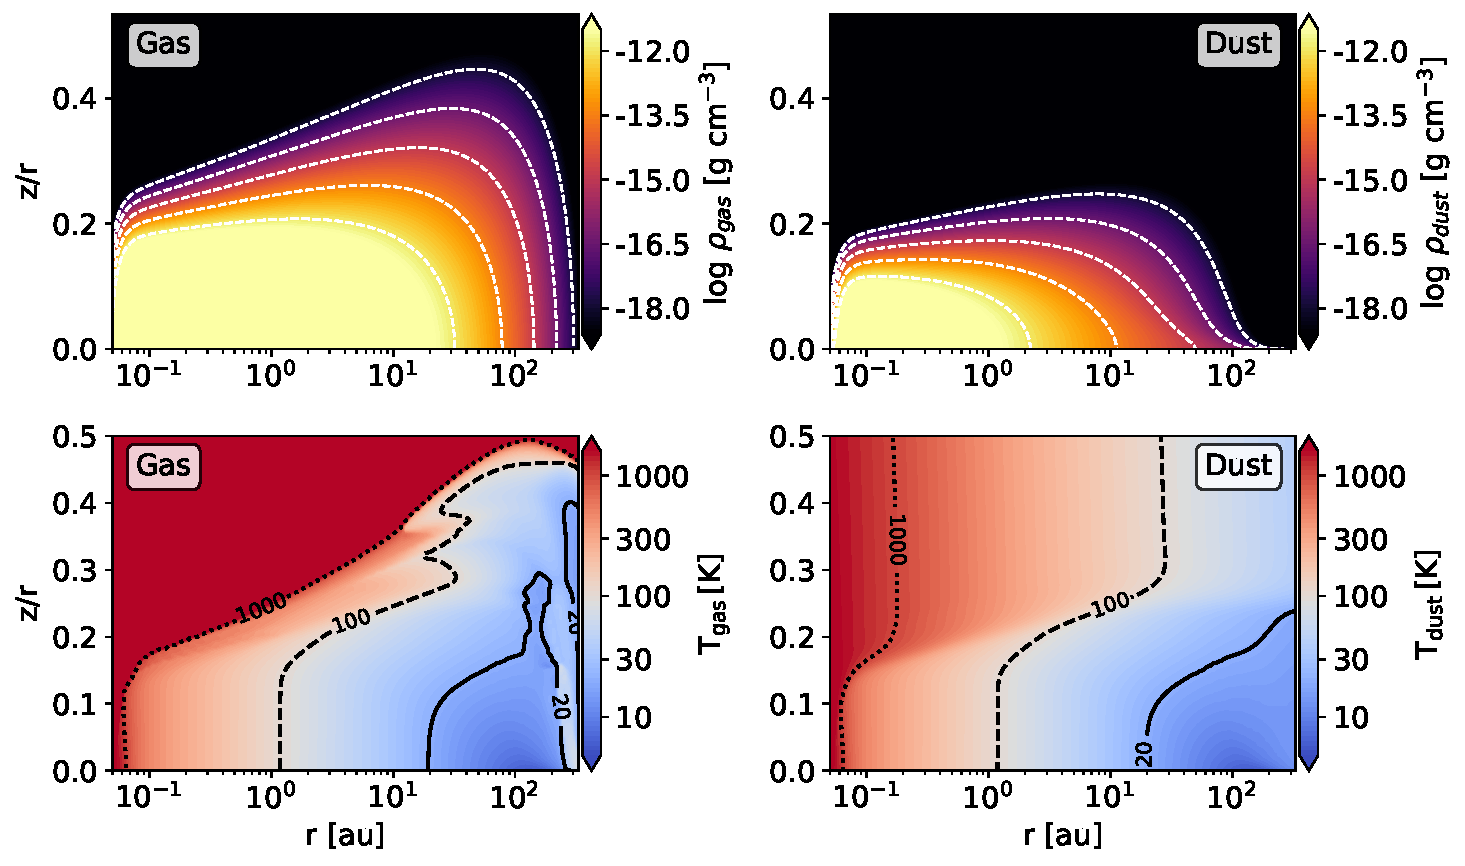
\includegraphics[width=\linewidth]{Figures/DensityTemperature.pdf}
    \caption{The density and temperature maps of gas and dust in the disk of the fiducial model. The horizontal axis shows the distance $r$ from the host star, and the vertical axis shows the height above the midplane $z$ divided by the radius $r$.}
    \label{fig: tempdensity}
\end{figure}
\textbf{COMPARING NON-ENHANCED TO ENHANCED}
After running the models, we analyzed their output. First, we looked at the densities of the gas and dust in the disk. The densities of the fiducial model are shown in the top row of \autoref{fig: tempdensity}. The density of the gas is more vertically extended than the density of the dust. This is expected, as the dust settles around the midplane. Furthermore, the gas density stretches farther from the host star than the dust. 

Next, we inspected the temperatures of gas and dust across the disk. Those are shown in the bottom row of \autoref{fig: tempdensity}.  The gas and dust temperatures vary across the disk for different heights and radii. However, they are equal in the midplane as they are coupled. Above the midplane, they decouple, and the temperatures of the gas and dust change. The gas temperatures are higher as they get heated by the star, whereas the dust temperatures are lower. Notably, the temperature of the dust is vertically isothermal. This result is expected as the density of the dust is orders of magnitude lower than that of the gas in the upper regions of the disk.  As a result, starlight passes through with minimal obstruction, leading to little variation in temperature with height.

% \begin{figure}[H]
%     \centering
%     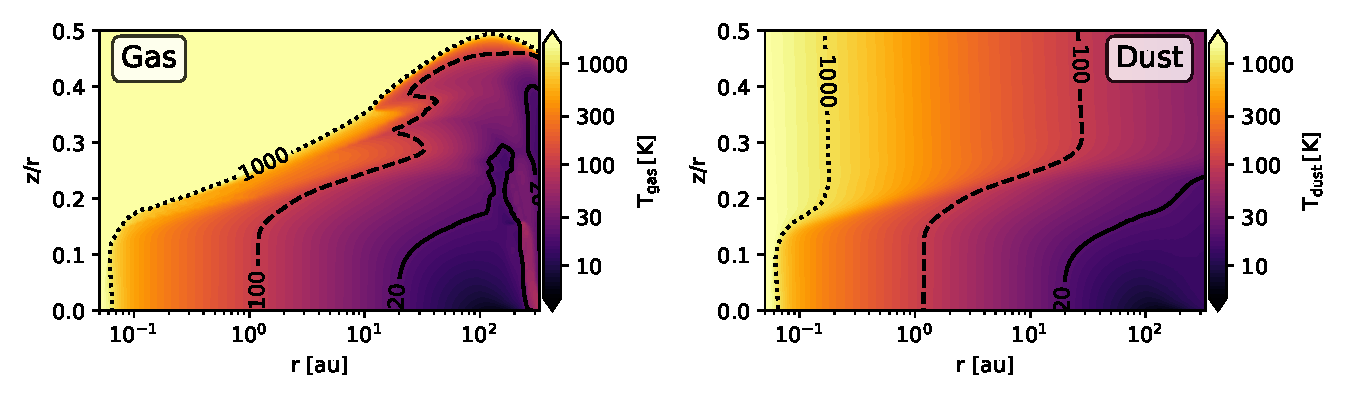
\includegraphics[width=\linewidth]{Figures/Temperature.pdf}
%     \caption{The temperature profile of gas and dust in the disk of the fiducial model.}
%     \label{fig: temperature}
% \end{figure}


\begin{figure}[H]
    \centering
    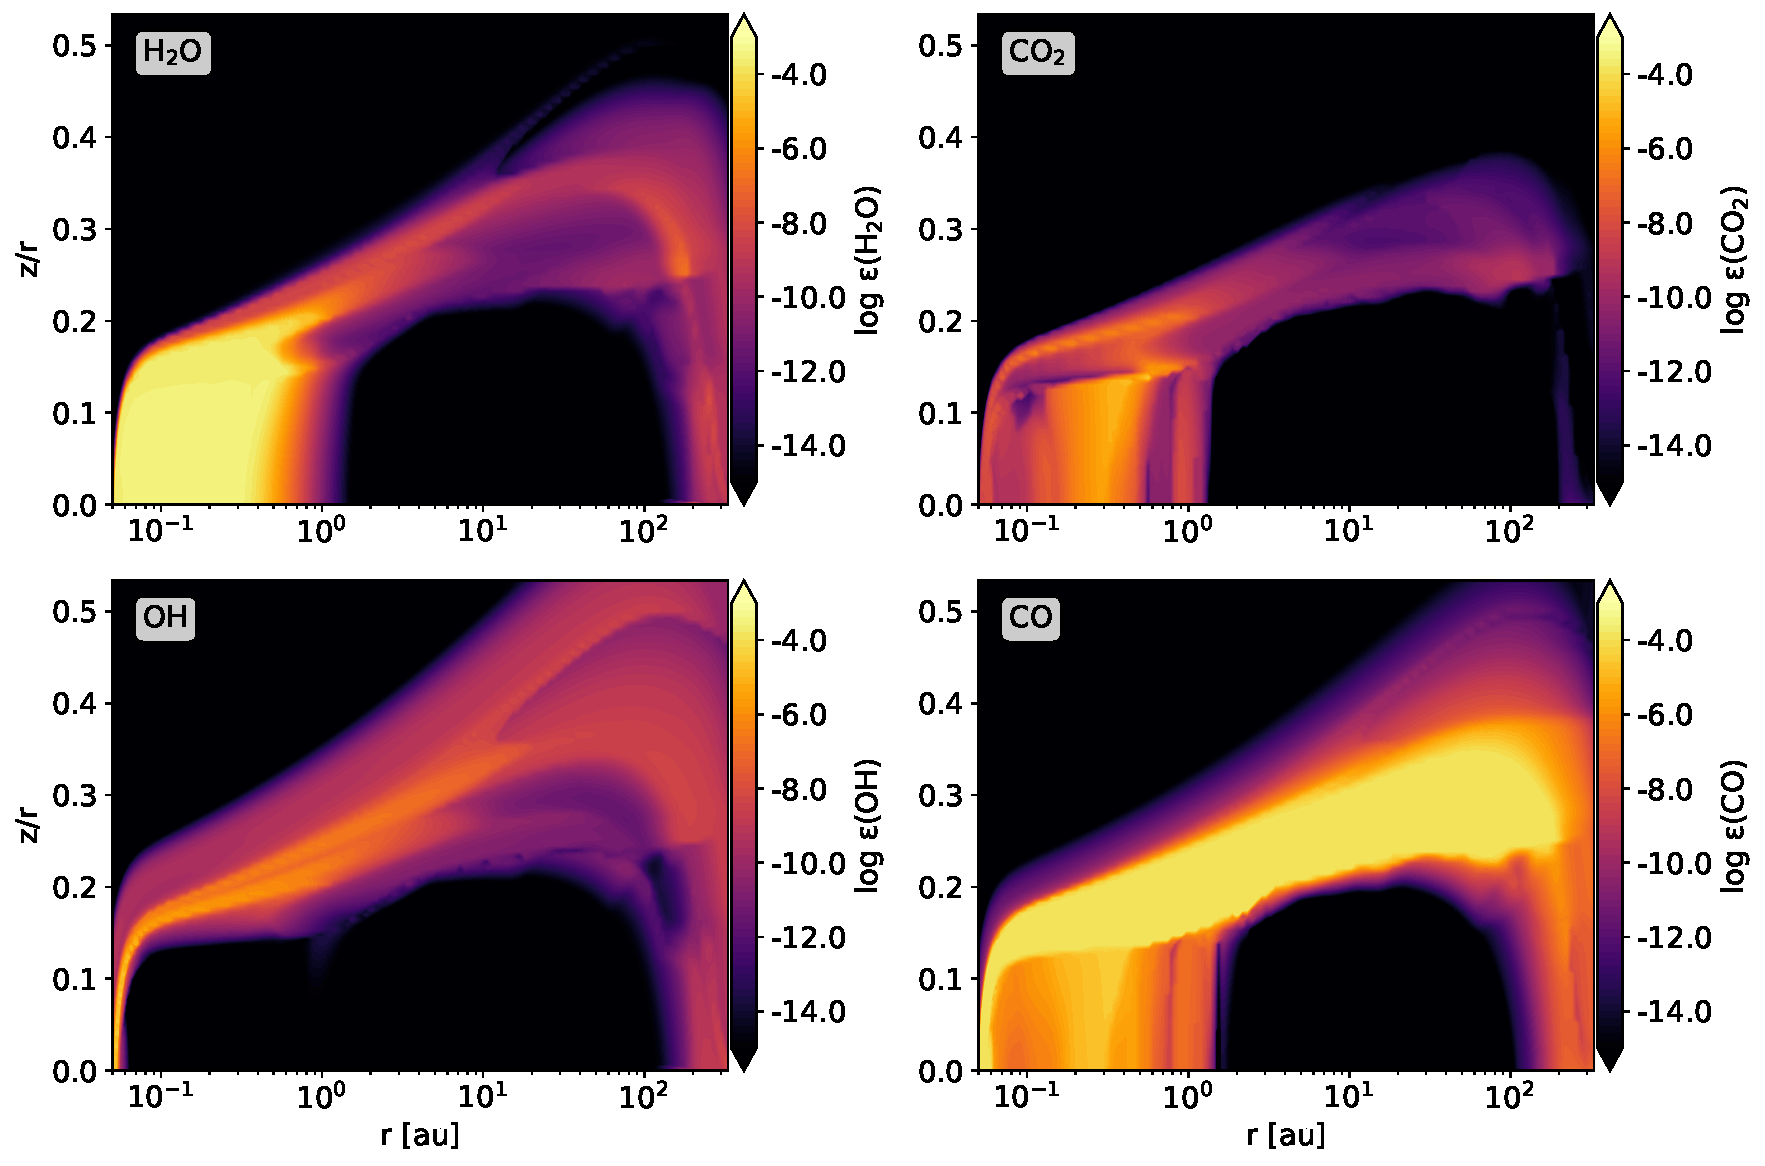
\includegraphics[width=\linewidth]{Figures/Abundance1.pdf}
    \caption{The distribution of H\2O, CO\2, OH, and CO across the disk of the fiducial model. The horizontal axis shows the distance $r$ from the host star, and the vertical axis shows the height above the midplane $z$ divided by the radius $r$.}
    \label{fig: others distribution}
\end{figure}

\begin{figure}[H]
    \centering
    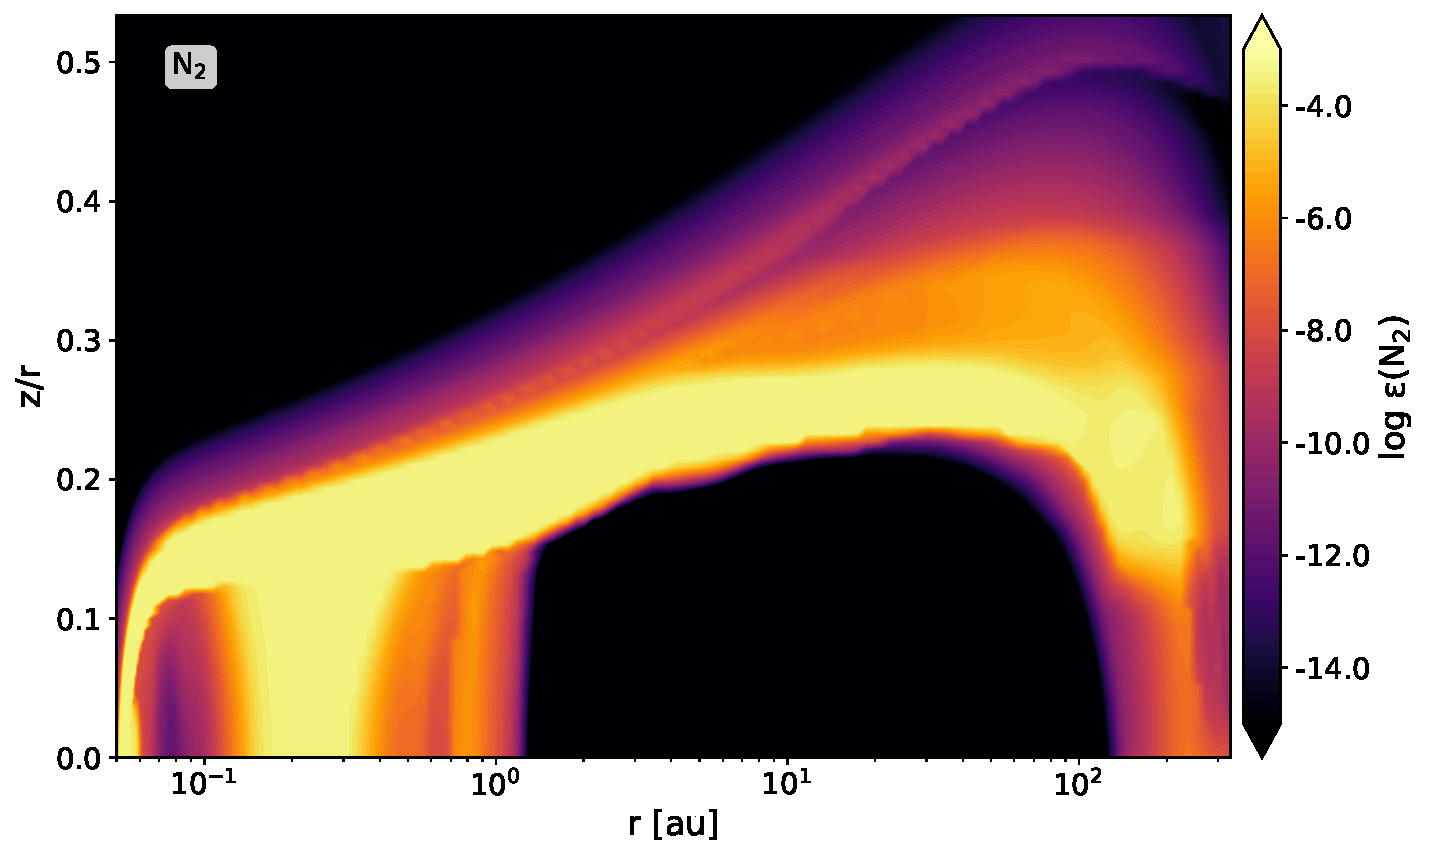
\includegraphics[width=.8\linewidth]{Figures/AbundanceN2.pdf}
    \caption{The distribution of N\2 across the disk of the fiducial model. The horizontal axis shows the distance $r$ from the host star, and the vertical axis shows the height above the midplane $z$ divided by the radius $r$.}
    \label{fig: n2 distribution}
\end{figure}

\begin{figure}[H]
    \centering
    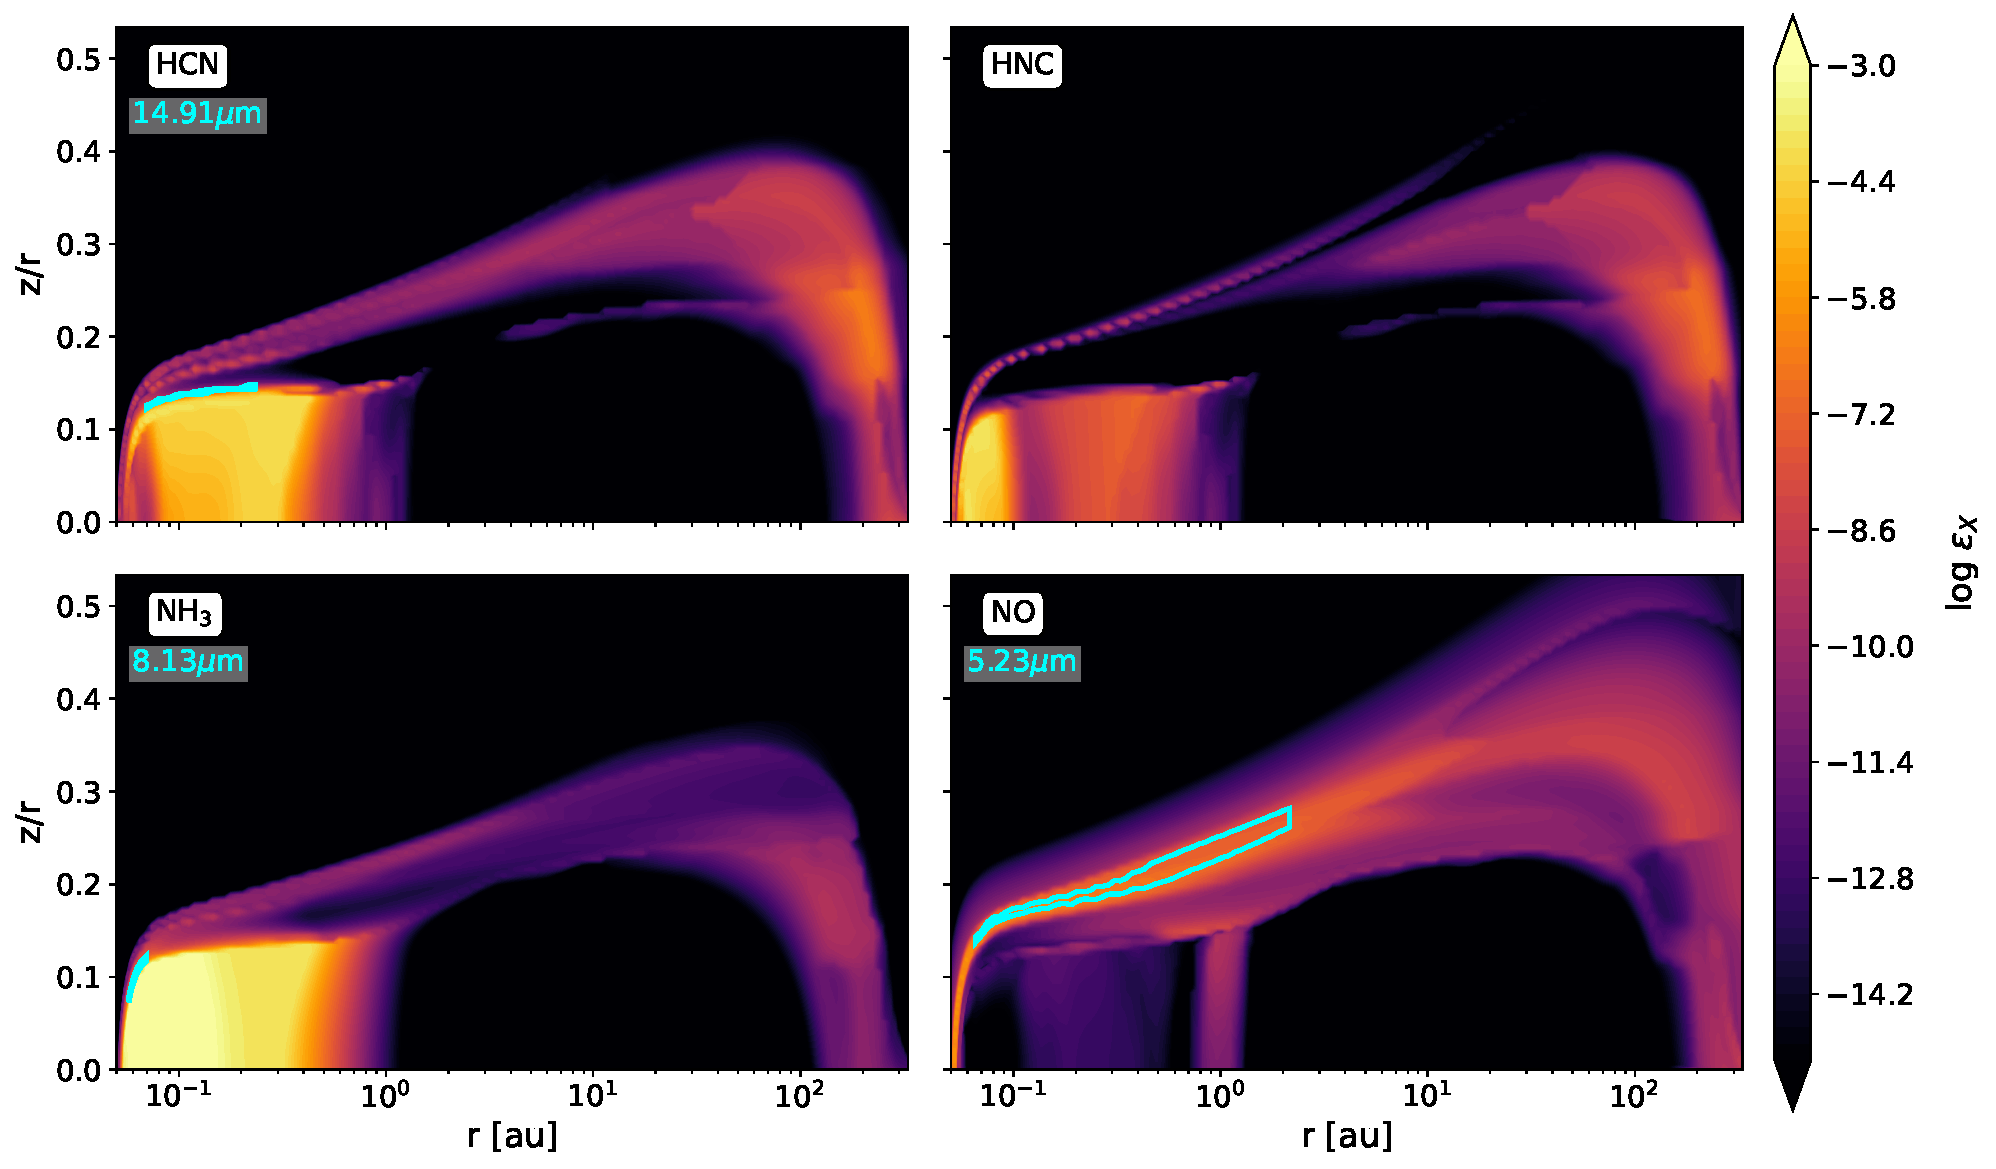
\includegraphics[width=\linewidth]{Figures/Abundance2.pdf}
    \caption{The distribution of HCN, HNC, NH\3, and NO across the disk of the fiducial model. The horizontal axis shows the distance $r$ from the host star, and the vertical axis shows the height above the midplane $z$ divided by the radius $r$.}
    \label{fig: nitrogen distribution}
\end{figure}
Lastly, we inspected the distribution of nitrogen-bearing molecules: N\2 (\autoref{fig: n2 distribution}), HCN, HNC, NH\3, and NO (\autoref{fig: nitrogen distribution}). The density of the molecules changes a lot for different radii and heights. For example, in the region between 0.05 and 0.1 au, HCN decreases compared to the surrounding areas, but HNC increases in the same region. There is a gap in the densities between 1 and 200 au. In these areas, the temperature drops below the freezing point of these molecules, and they are well shielded from UV radiation, resulting in the formation of ice. 
% \newpage
\section{FLiTs Spectra}
Consistent mid-infrared spectra were calculated using FLiTs for all the models in the grid. The resulting spectra are shown in \autoref{fig: all spectra}. There is a clear division in the shapes of the spectra. In the bottom left corner, 6 spectra have a strong C\2H\2 feature. These models also have a C/O ratio greater than unity. The other models have strong water features and have a C/O ratio smaller than unity. 

\begin{figure}[H]
    \centering
    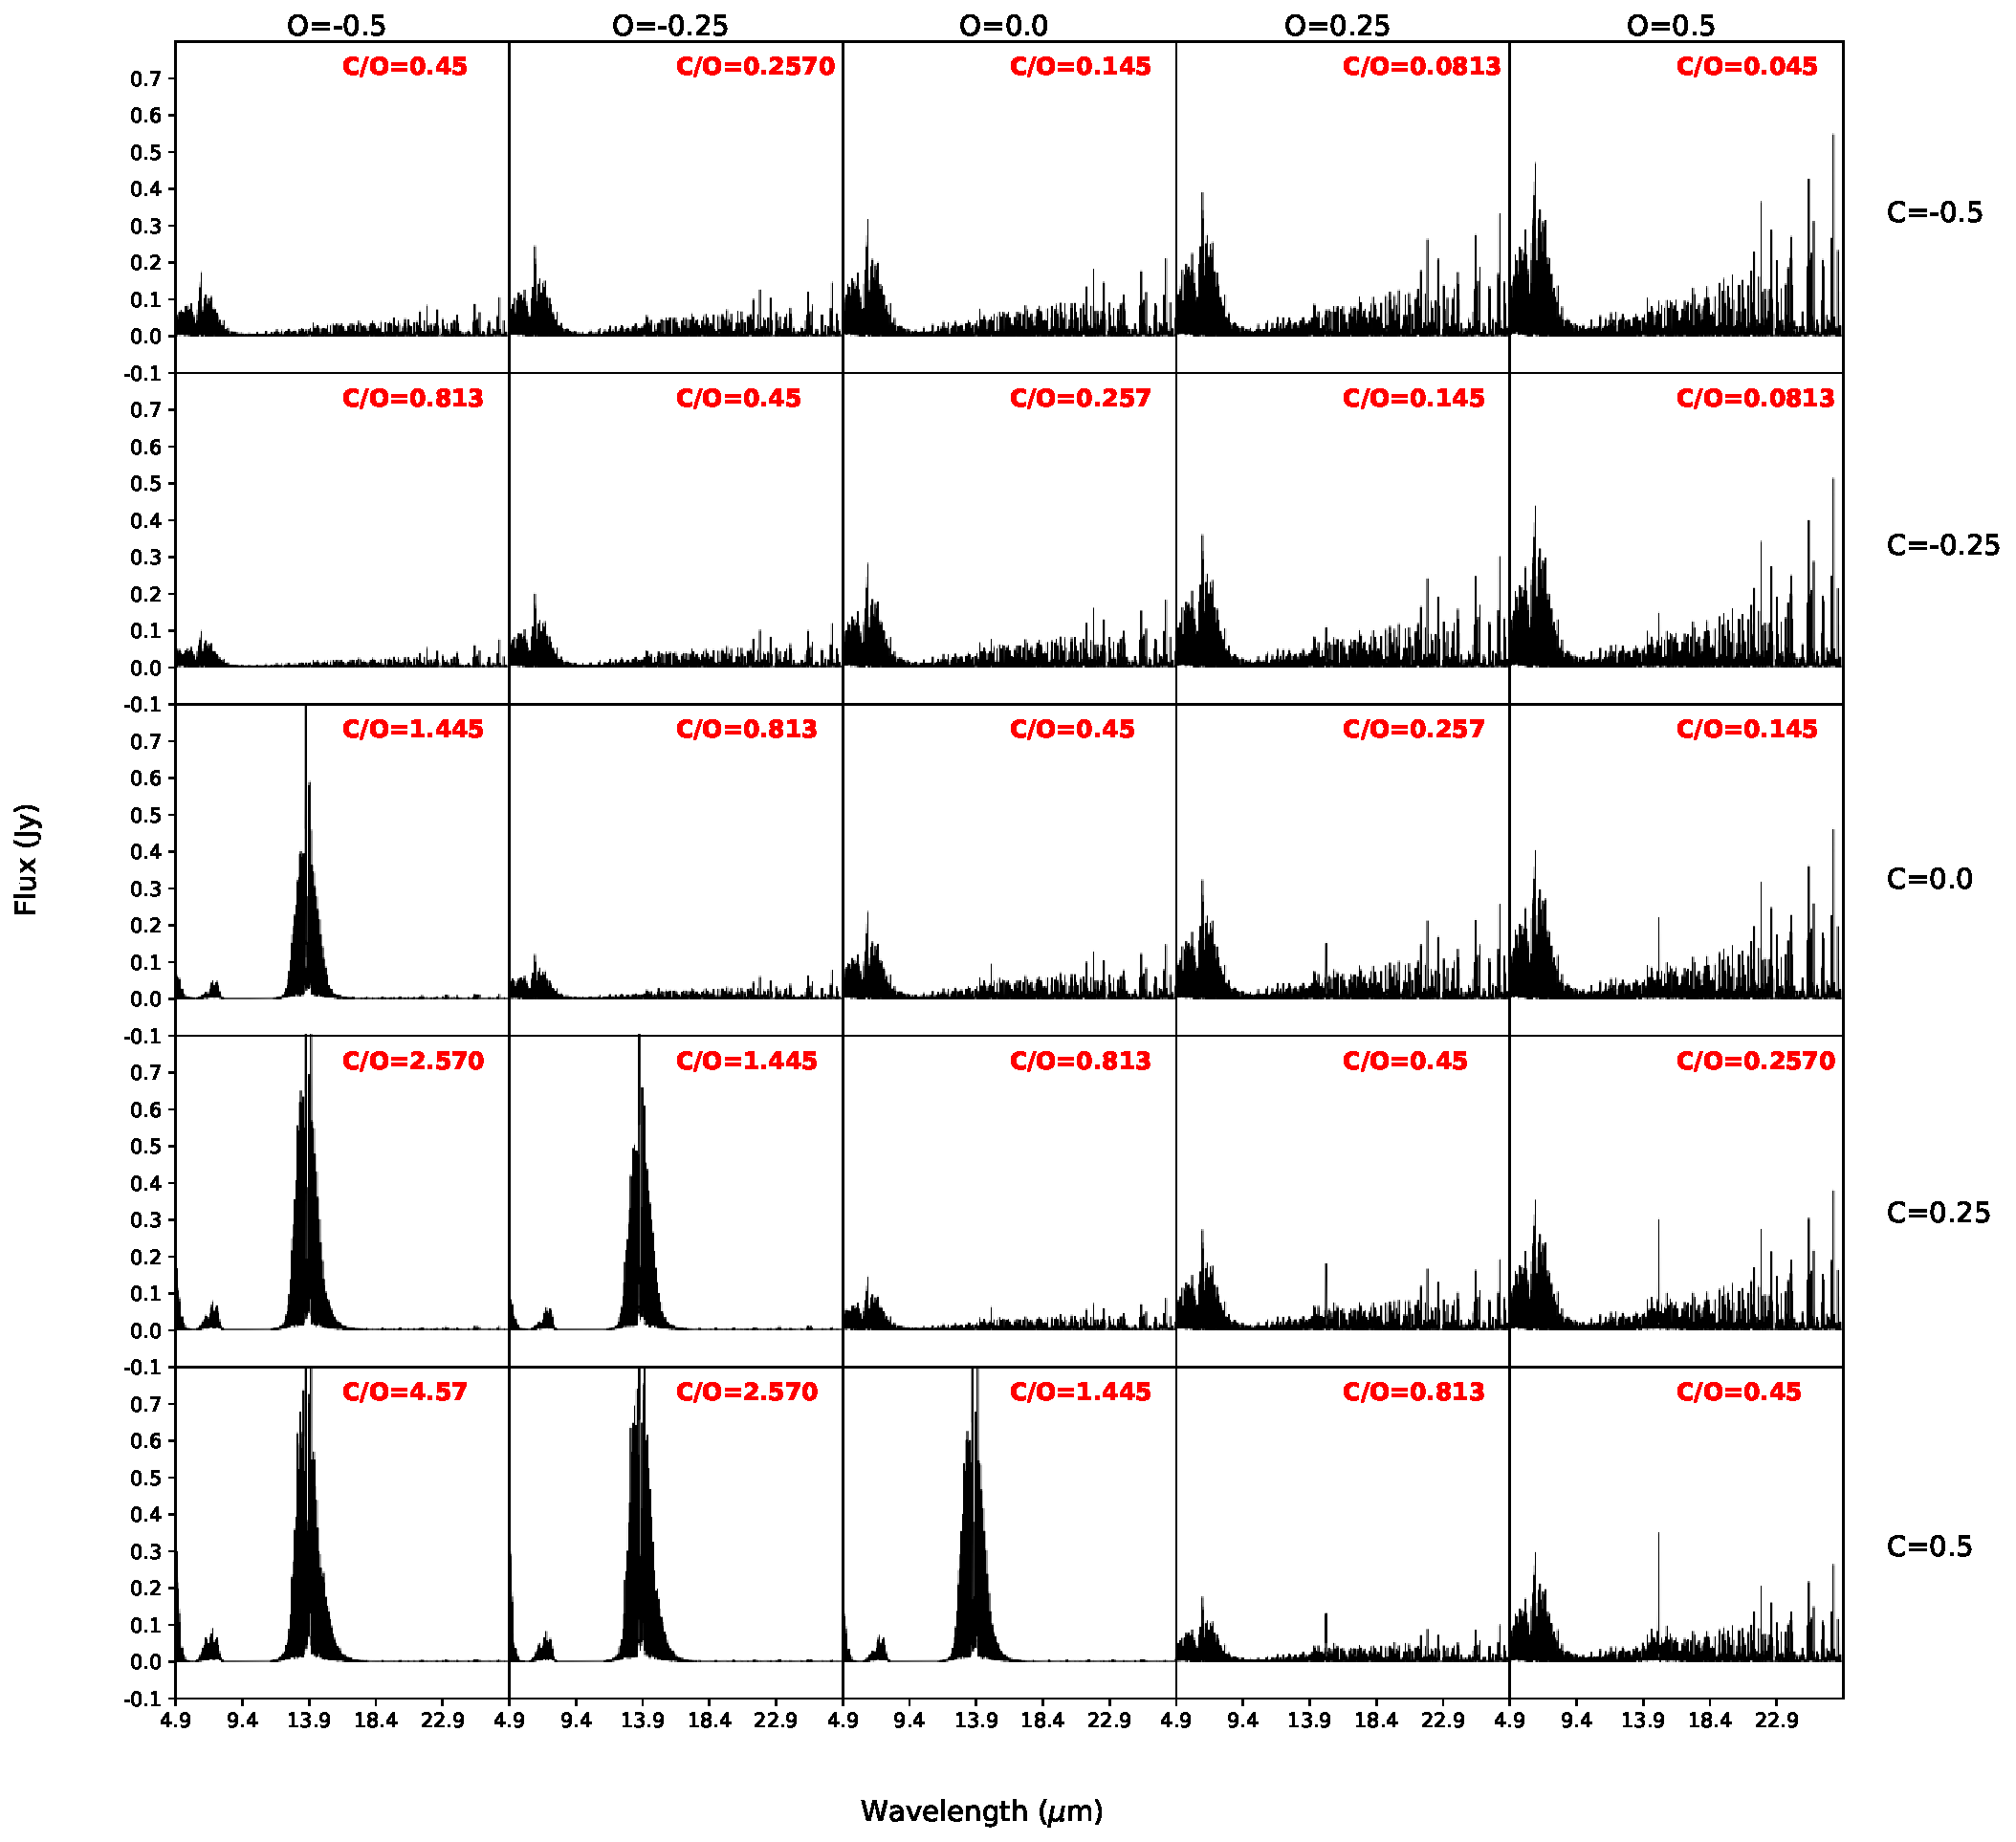
\includegraphics[width=\linewidth]{Figures/All_spectra.pdf}
    \caption{The simulated spectra of all the models in the model grid using FLiTs. On the horizontal axis, the O abundance is varied from -0.5 to 0.5 w.r.t. the reference abundance. The C abundance is varied with -0.5 to 0.5 w.r.t. the reference abundance from top to bottom.}
    \label{fig: all spectra}
\end{figure}
\subsection{Total Flux across Grid}
The flux of the different species changes depending on the abundances of C and O. \autoref{fig: Heatmaps1} shows the total flux for CO, CO\2, H\2O, and OH across the grid of models. The total flux for C\2H\2, HCN, NO, and NH\3 for all the models in the grid is shown in \autoref{fig: Heatmaps2}. 

\begin{figure}[H]
    \centering
    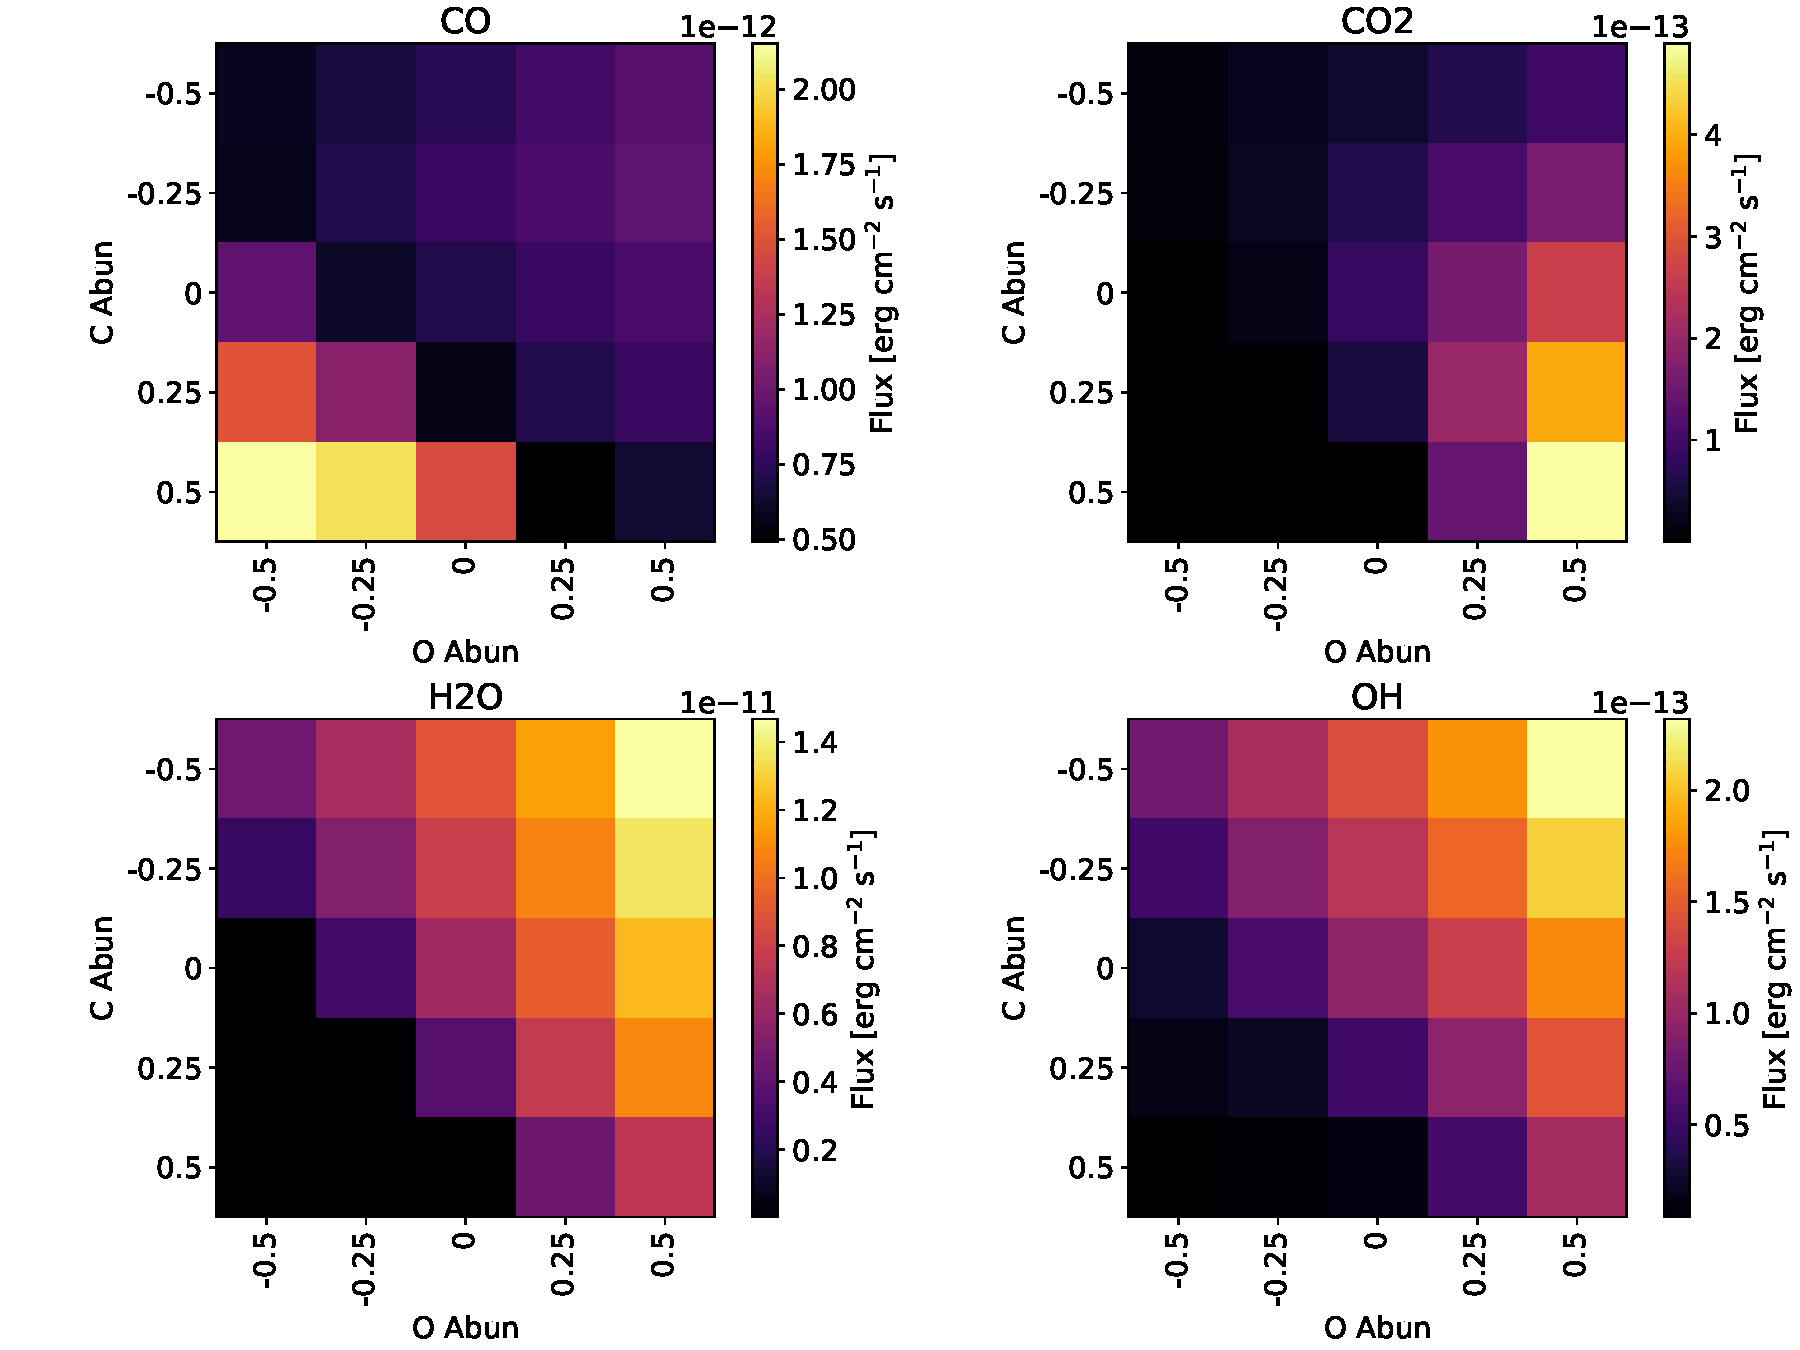
\includegraphics[width=\linewidth]{Figures/Heatmaps1.pdf}
    \caption{The total flux of CO, CO\2, H\2O, and OH for all the models in the grid.}
    \label{fig: Heatmaps1}
\end{figure}
\begin{figure}[H]
    \centering
    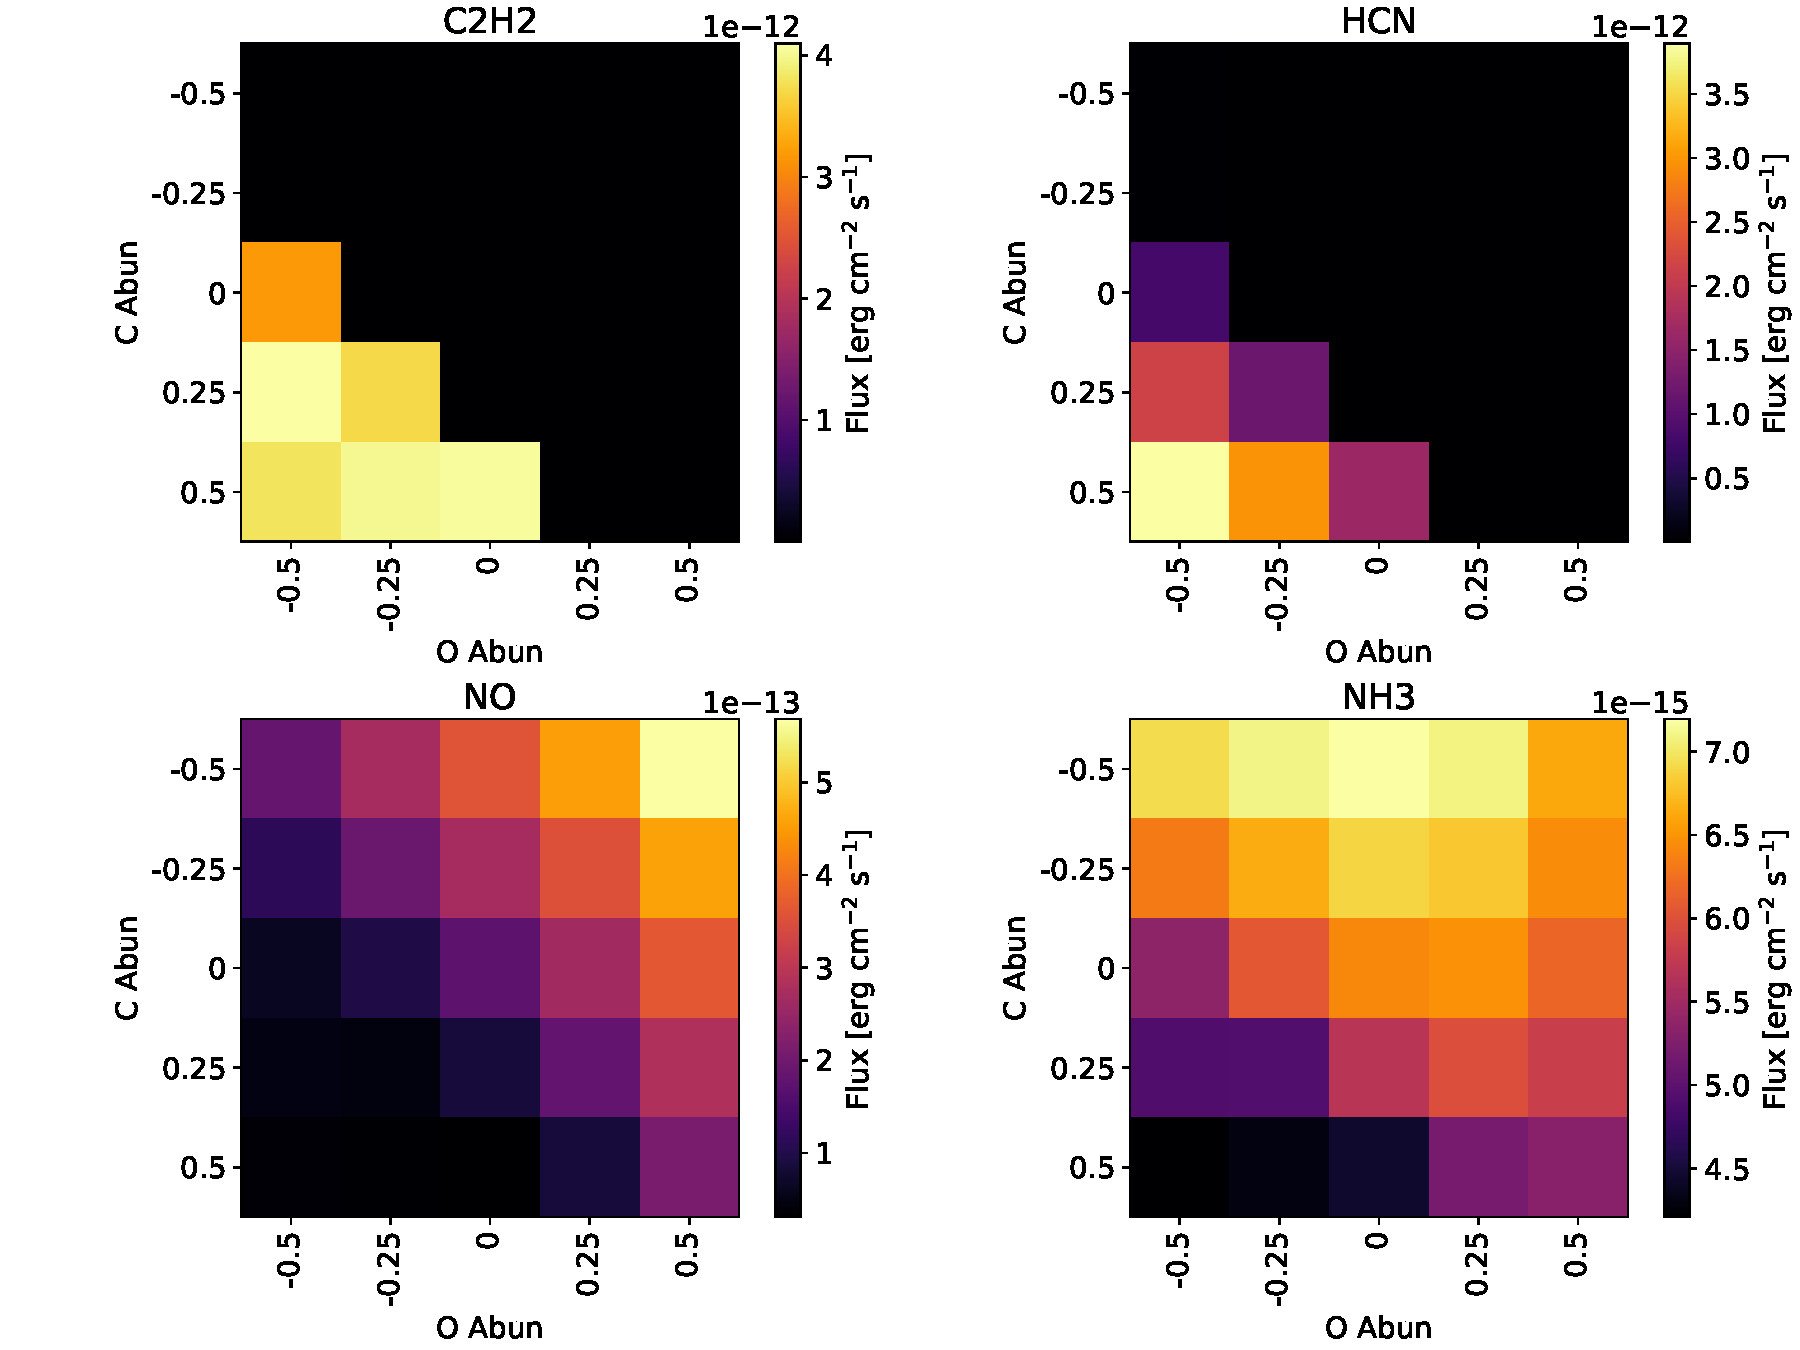
\includegraphics[width=\linewidth]{Figures/Heatmaps2.pdf}
    \caption{The total flux of C\2H\2, HCN, NO, and NH\3 for all the models in the grid.}
    \label{fig: Heatmaps2}
\end{figure}

The HCN flux increases as C/O gets larger, and NO decreases. The flux of NH\3 generally increases as the C abundance gets lower. We hypothesize that the cause for this is the reactions that take place to form NH\3.
OH is an important component in the formation of NH\3. \textbf{CHECK CHEMISTRY}

\ce{NH2+ + OH -> NH3 + O+}

\textbf{MORE REACTIONS}\\
Furthermore, there could be some competition with HCN, where more N is locked in HCN when the C abundance is larger. 

\subsection{Regions of Interest}
Next, we wanted to identify regions in the spectrum that could help us detect NO and NH\3. We split the model grid into 2 groups. One group has C/O smaller than unity, and the other greater. We chose this distinction as the behaviors of the spectra are different. This difference is also visible in \autoref{fig: all spectra}. 

% \begin{figure}[H]
%     \centering
%     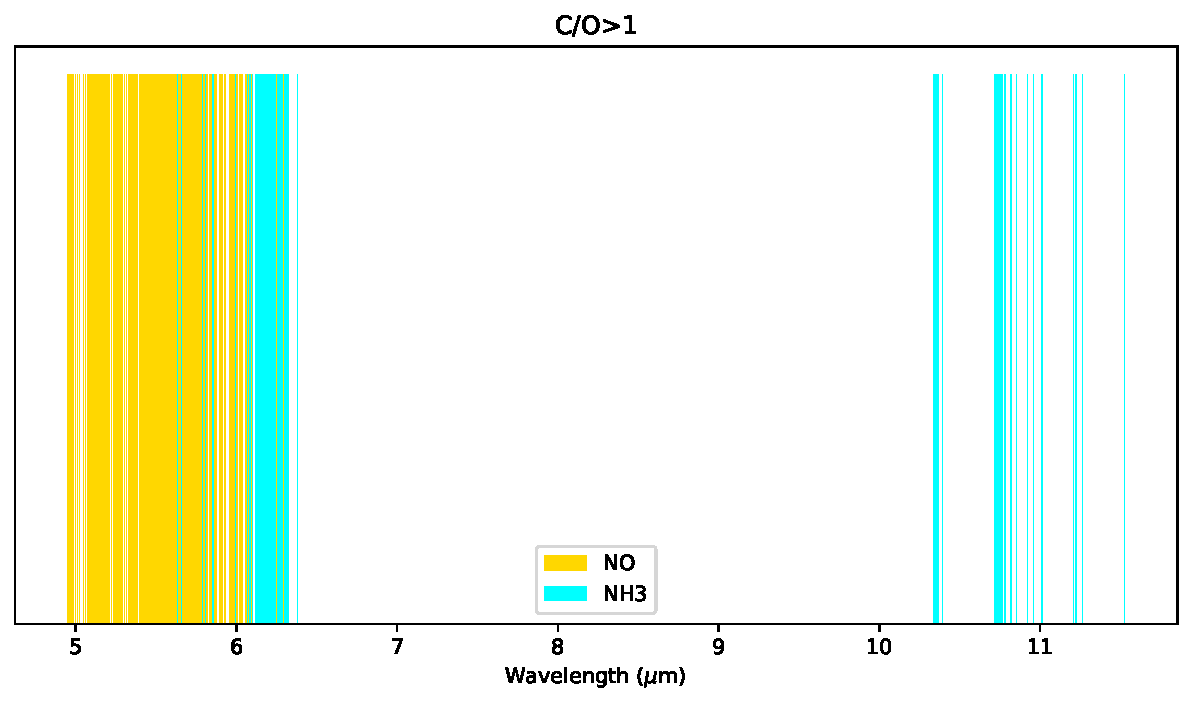
\includegraphics[width=\linewidth]{Figures/ClassificationCOgt0.pdf}
%     \caption{The regions of the spectrum where NO and NH\3 emission are the  strongest compared to other molecular emission in the models that have a C/O greater than unity}
%     \label{fig: class>1}
% \end{figure}

% \begin{figure}[H]
%     \centering
%     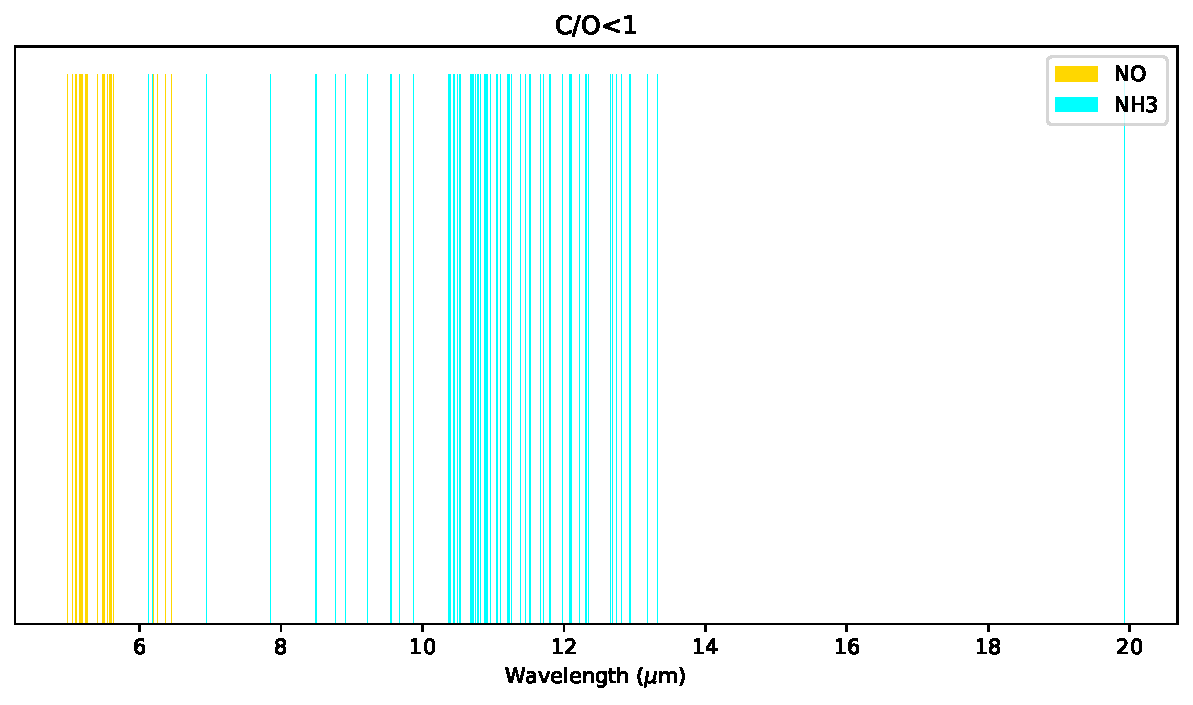
\includegraphics[width=\linewidth]{Figures/ClassificationCOst0.pdf}
%     \caption{The regions of the spectrum where NO and NH\3 emission are strongest in the models that have a C/O smaller than unity}
%     \label{fig: class<1}
% \end{figure}

\begin{figure}[H]
    \centering
    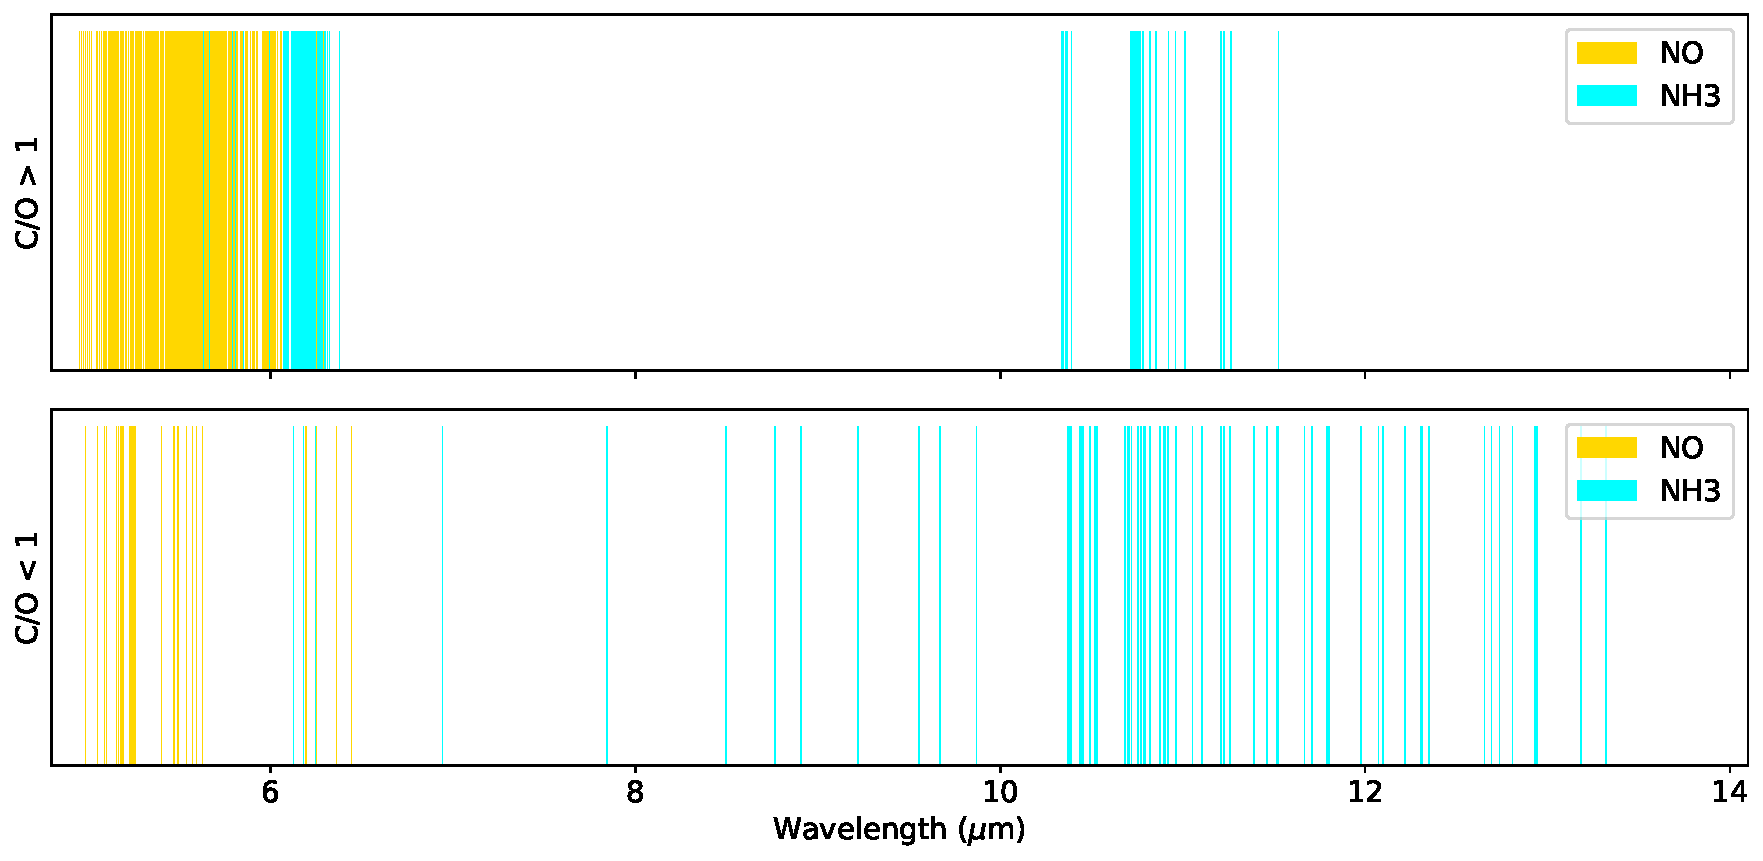
\includegraphics[width=\linewidth]{Figures/ClassificationCO.pdf}
    \caption{The regions of the spectrum where NO and NH\3 emission are strongest in the models that have a C/O smaller than unity}
    \label{fig: classes}
\end{figure}

In the top row of \autoref{fig: classes}, it is visible that the region between 4.9$\mu$m and 6 $\mu$m has many spectral regions where NO emission is strongest. NH\3 has the brightest emission compared to all the other molecules between 6 $\mu$m and 6.4 $\mu$m. Between 10 $\mu$m and 12 $\mu$m there are some smaller regions where NH\3 is strongest. In contrast, in the bottom row of \autoref{fig: classes}, the spectral regions where NO or NH\3 emission is strongest are more barren. The NO emission regions are not the strongest anymore, and neither is the NH\3 emission region next to it. The most promising region for NH\3 is now between 10 $\mu$m and 12 $\mu$m. 

\begin{figure}[H]
    \centering
    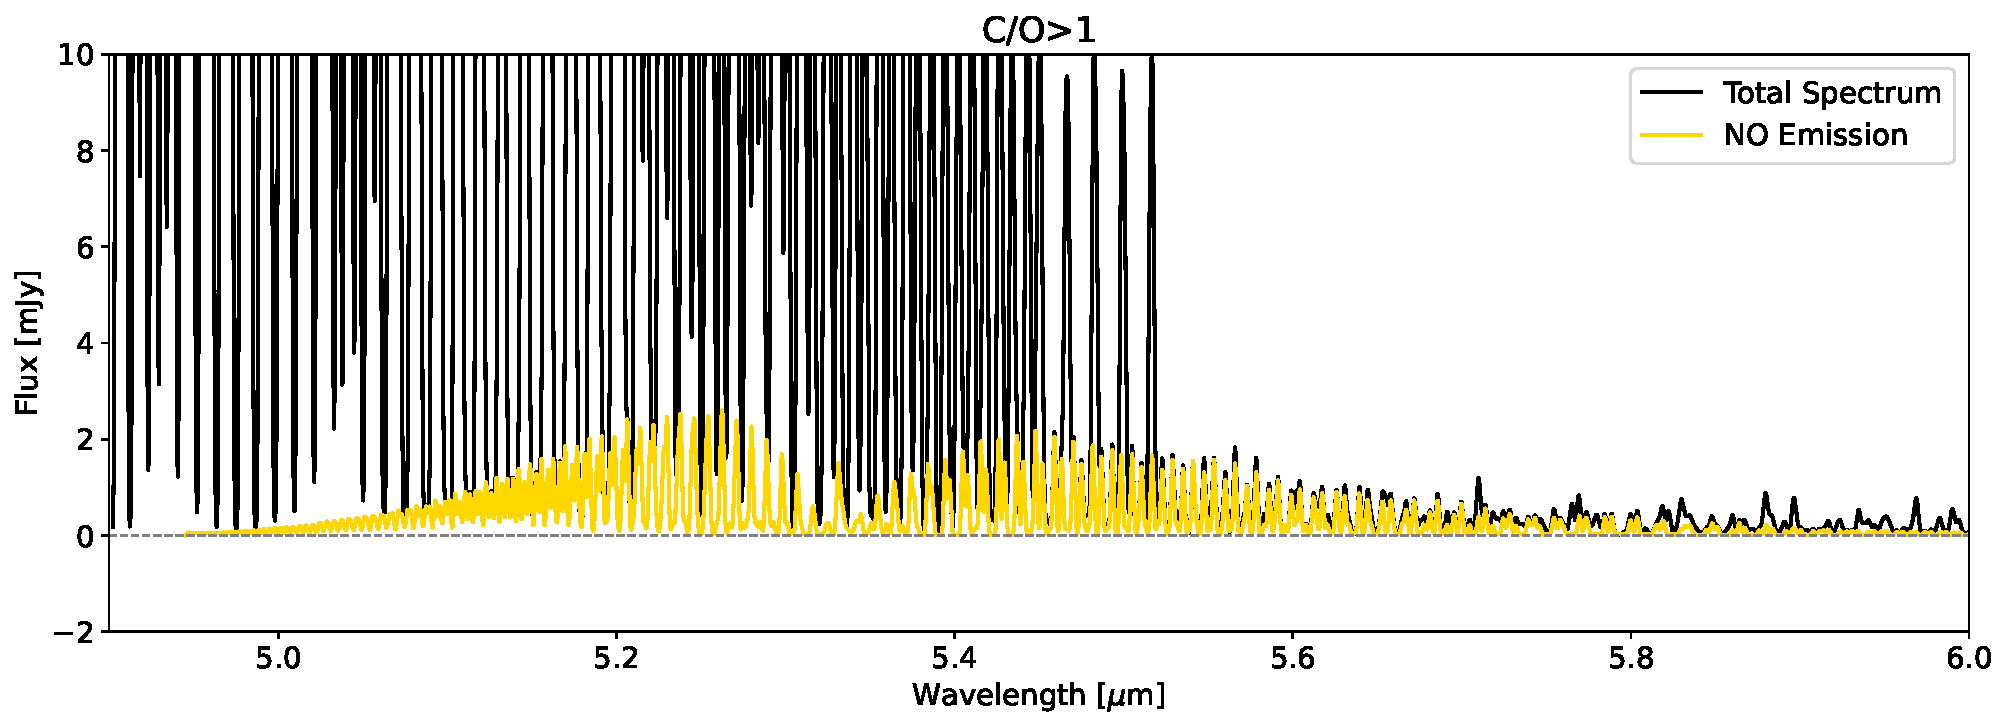
\includegraphics[width=\linewidth]{Figures/NO_region.pdf}
    \caption{A zoomed-in region of the spectrum of the fiducial model between 4.9 $\mu$m and 6 $\mu$m where NO emission is strongest.}
    \label{fig: NO region}
\end{figure}



\begin{figure}[H]
    \centering
    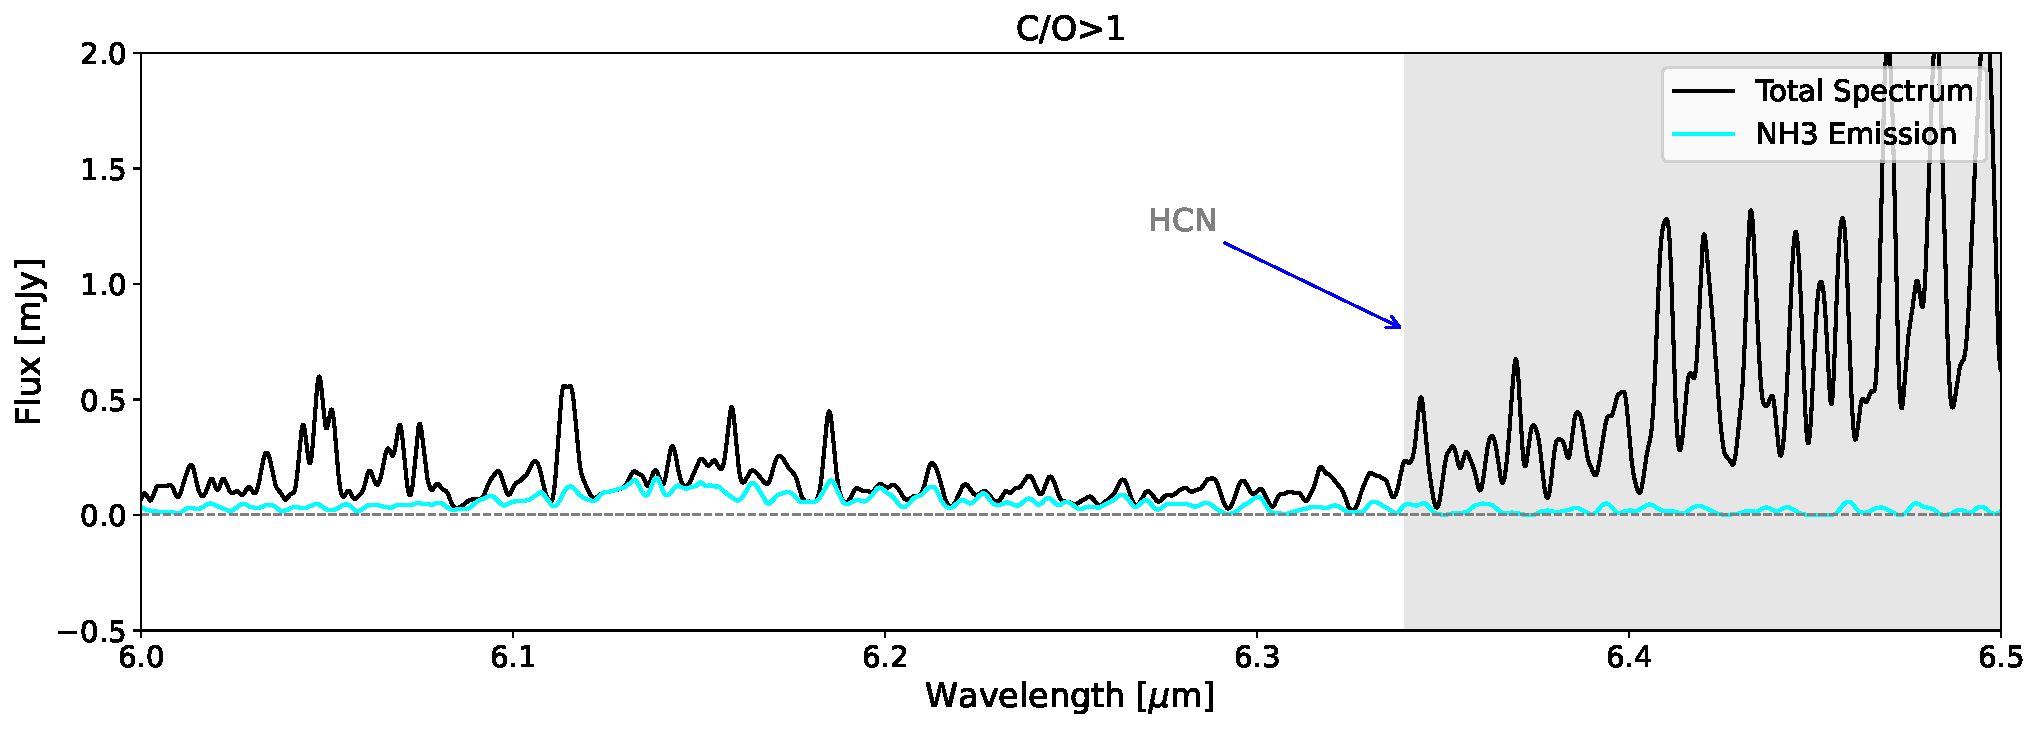
\includegraphics[width=\linewidth]{Figures/NH3_region1.pdf}
    \caption{A zoomed-in region of the spectrum of the model with C+0.25 and O-0.25 between 6 $\mu$m and 6.5 $\mu$m where NH\3 emission is strongest.}
    \label{fig: NH3 region 1}
\end{figure}
\begin{figure}[H]
    \centering
    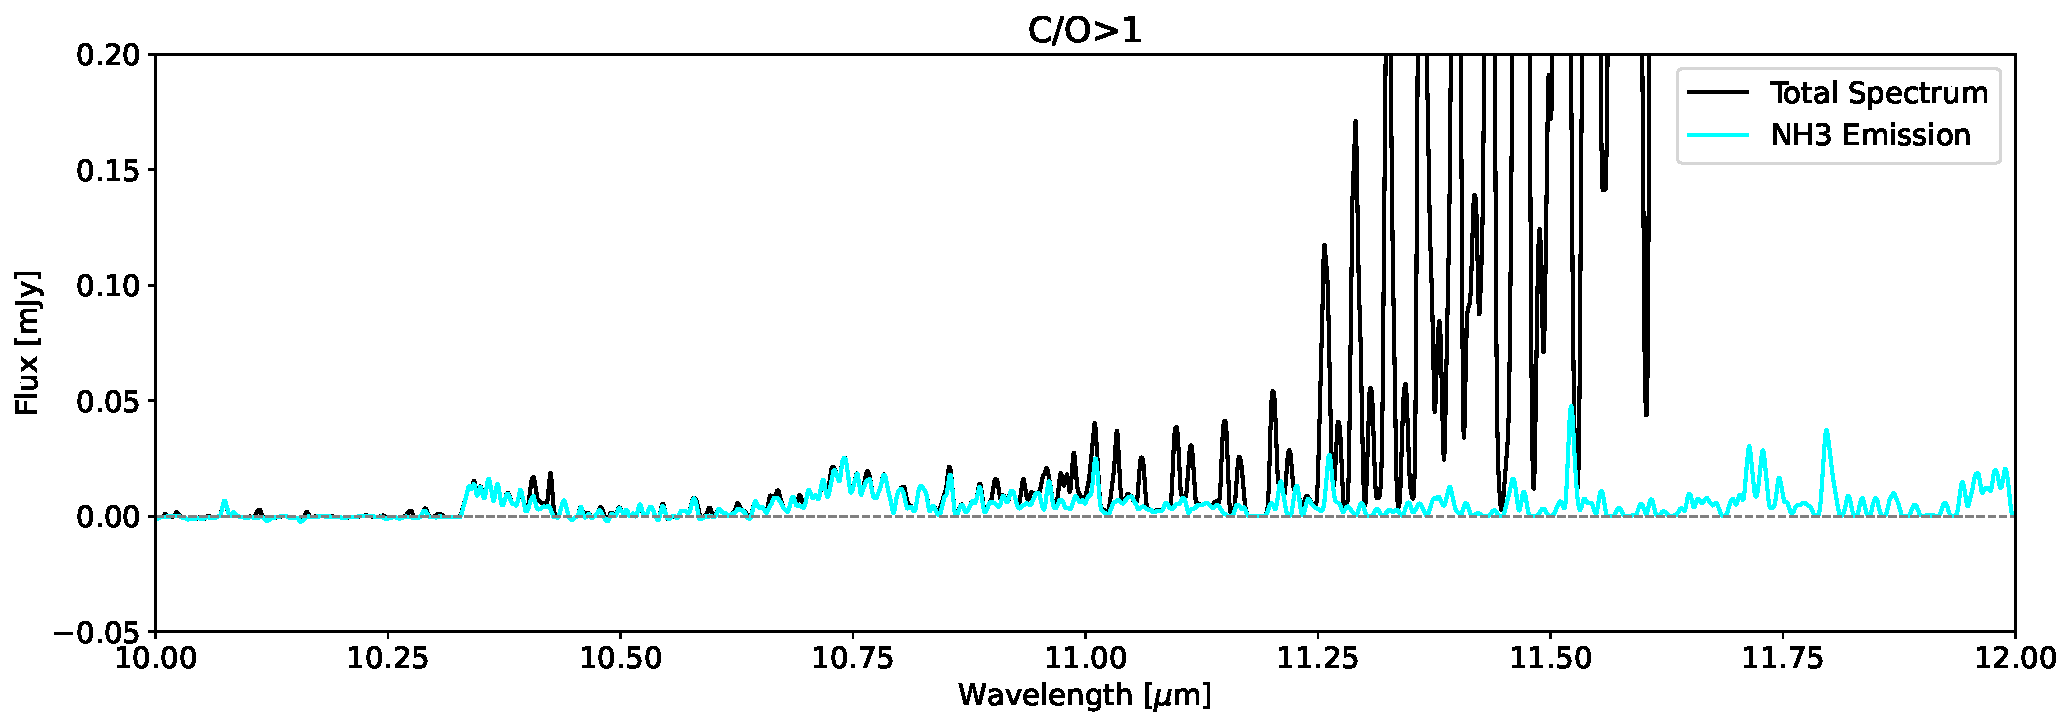
\includegraphics[width=\linewidth]{Figures/NH3_region2.pdf}
    \caption{A zoomed-in region of the spectrum of the model with C+0.25 and O-0.25 between 10 $\mu$m and 12 $\mu$m where NO emission is strongest.}
    \label{fig: NH3 region 2}
\end{figure}
\begin{figure}[H]
    \centering
    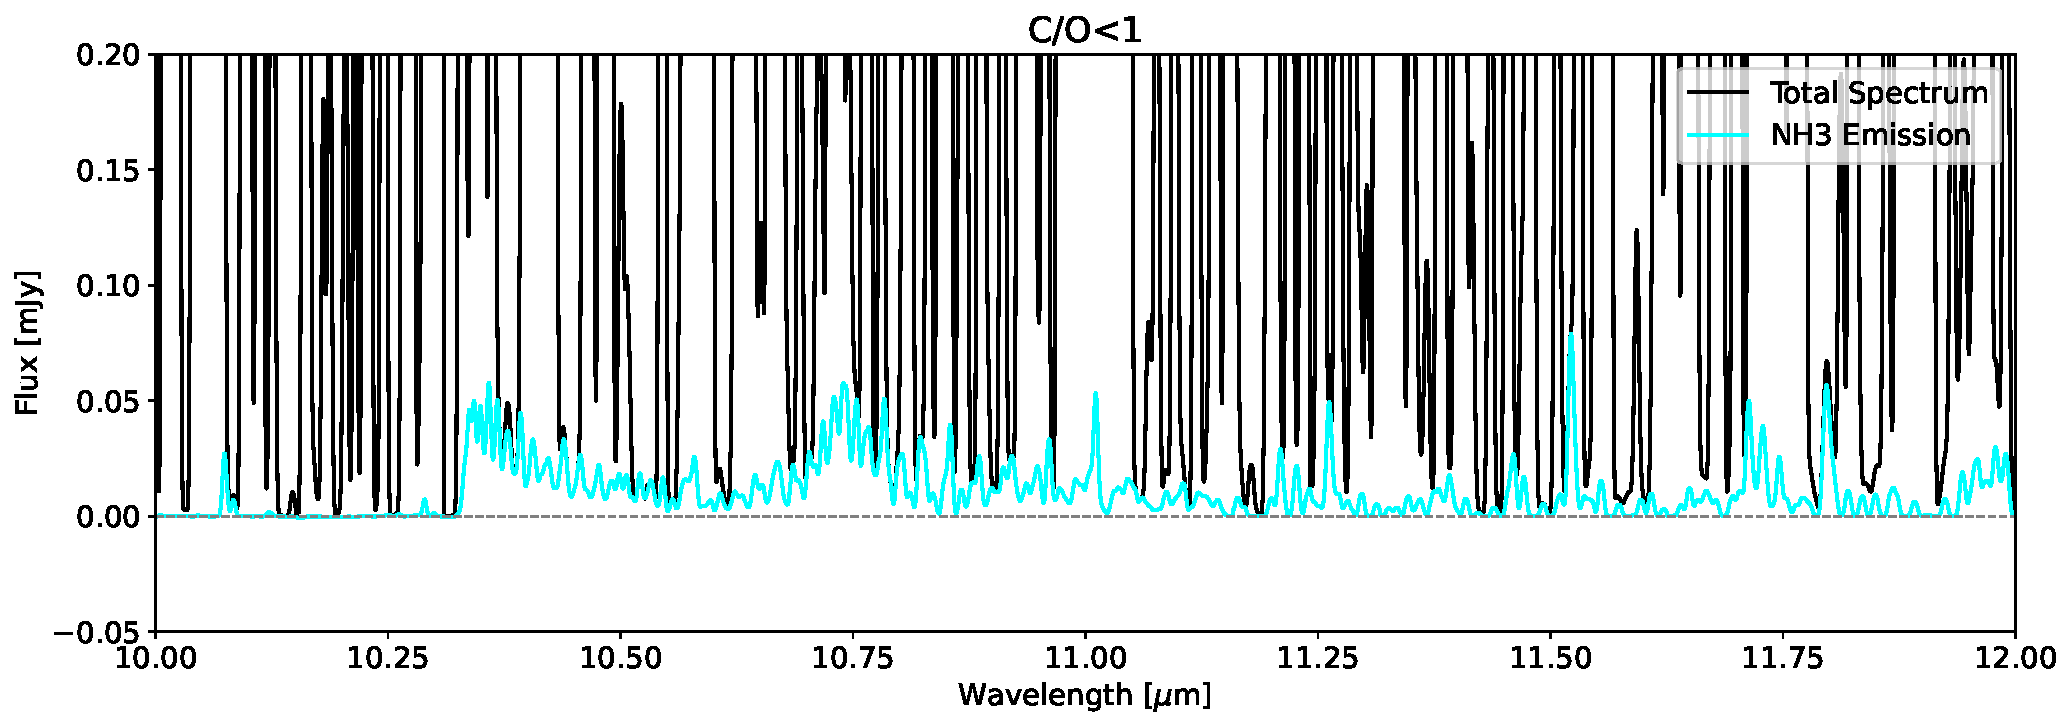
\includegraphics[width=\linewidth]{Figures/NH3_region3.pdf}
    \caption{A zoomed-in region of the spectrum of the fiducial model between 10 $\mu$m and 12 $\mu$m where NO emission is strongest.}
    \label{fig: NH3 region 3}
\end{figure}

The spectra in \autoref{fig: NO region}, \autoref{fig: NH3 region 1}, \autoref{fig: NH3 region 2}, and \autoref{fig: NH3 region 3} are all without any noise. When we added noise with SNR=300 to the same spectrum shown in figure \autoref{fig: NH3 region 1}, based on the methods described, we got the spectrum shown in figure \autoref{fig: add noise}. In this figure, the emission of NH\3 is obscured by noise at this SNR, making it much more difficult to detect.  

\begin{figure}[H]
    \centering
    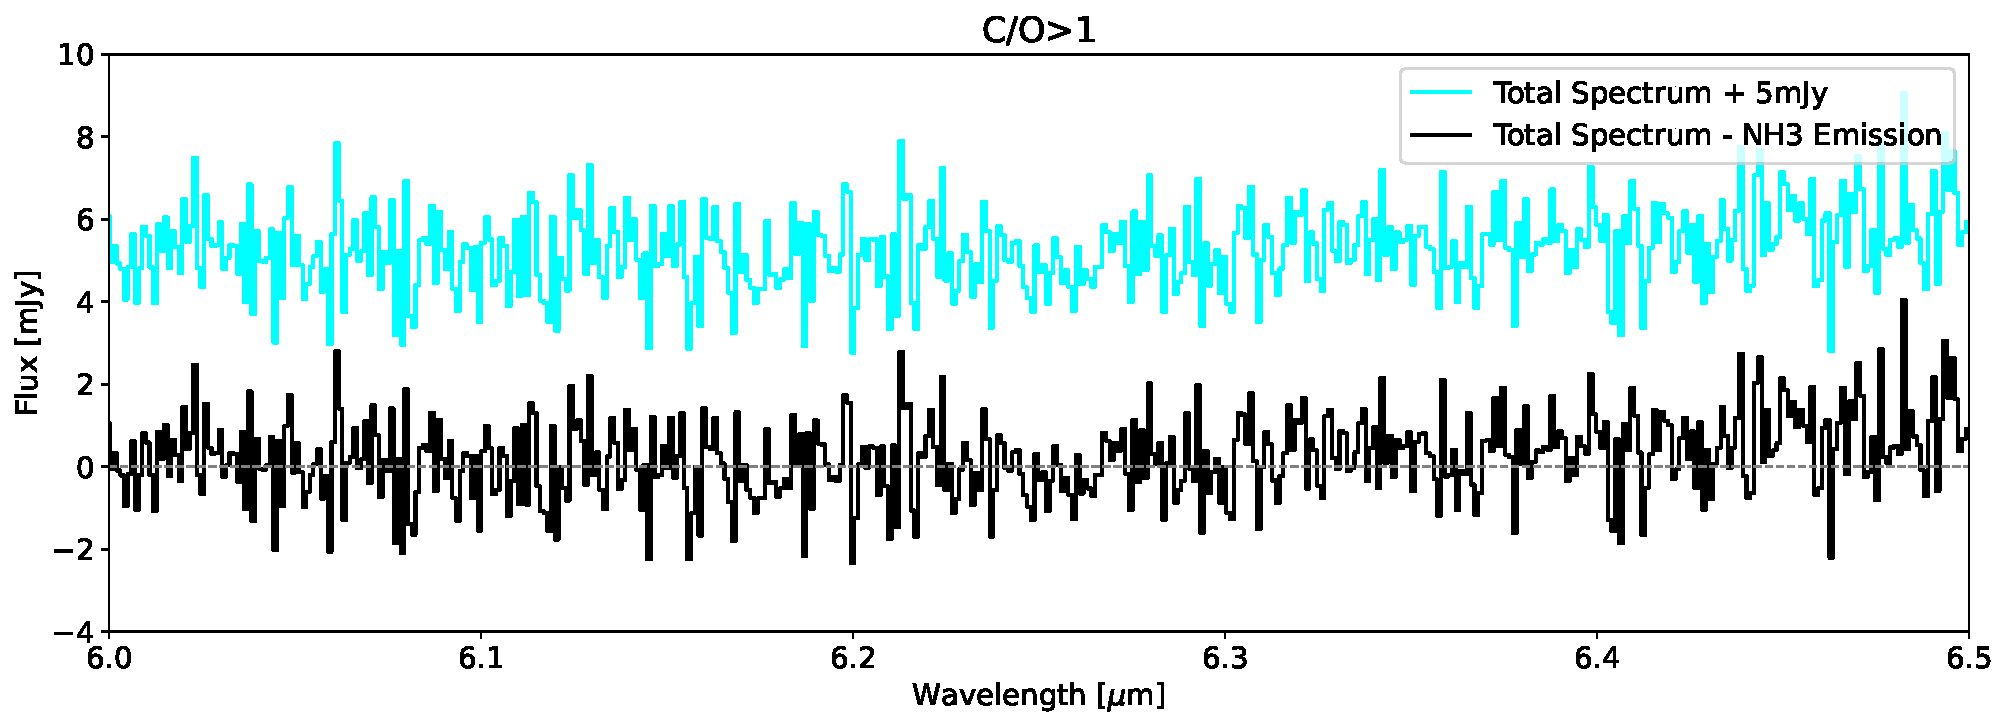
\includegraphics[width=\linewidth]{Figures/AddNoise.pdf}
    \caption{A zoomed-in region of the spectrum of the model with C+0.25 and O-0.25 between 6 $\mu$m and 6.5 $\mu$m where NH\3 emission is strongest. A Gaussian noise corresponding to an SNR of 300 was added.}
    \label{fig: add noise}
\end{figure}

\section{Molecule Detection}[!ht]
As visible in \autoref{fig: add noise}, it is hard to distinguish the NH\3 and NO from the spectrum visually. However, cross-correlation is a technique that can be used to find such weak signals. In calculating the cross-correlation, we used the average spectrum for each species of all the models in the model grid and normalized them. This template was then used to cross-correlate with the full spectrum. The cross-correlation of the H\2O template with the spectrum of the fiducial model is shown in \autoref{fig: crosscorr}. The peak signals that H\2O is present in the spectrum, and it indeed is present. 

\begin{figure}[H]
    \centering
    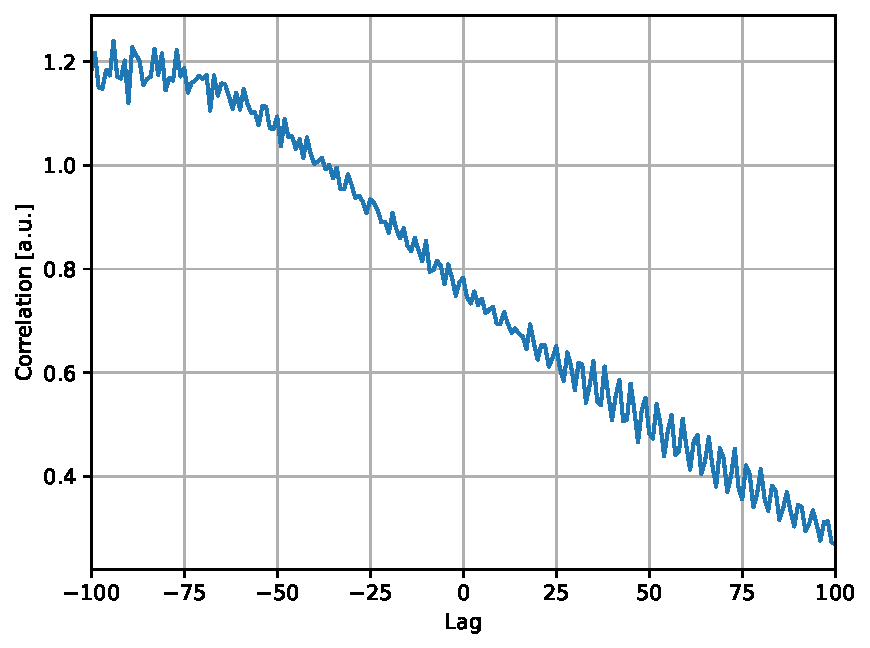
\includegraphics[width=.6\linewidth]{Figures/Cross-Correlation.pdf}
    \caption{The cross-correlation of the H\2O template with the spectrum the fiducial model}
    \label{fig: crosscorr}
\end{figure}

When we applied this method to the fiducial model and model C+0.25 O-0.25, we got the detections shown in \autoref{tab: combined_detections}. 

% \begin{table}[!ht]
% \centering
% \begin{tabular}{lll}
% \hline
% \textbf{Molecule} & \textbf{Spectrum} & \textbf{Spectrum - Target Flux} \\ \hline
% C\2H\2            & Non-detection     & Non-detection                   \\
% CH\4             & Non-detection     & Non-detection                   \\
% CO              & Detection         & Non-detection                   \\
% CO\2             & Detection         & Non-detection                   \\
% H\2O             & Detection         & Non-detection                   \\
% HCN             & Non-detection     & Non-detection                   \\
% NH\3             & Non-detection     & Non-detection                   \\
% NO              & Non-detection     & Non-detection                   \\
% OH              & Detection         & Non-detection                   \\ \hline
% \end{tabular}

% \label{tab: fiducial detection}
% \end{table}

% \begin{table}[!ht]
% \centering
% \begin{tabular}{lll}
% \hline
% \textbf{Molecule} & \textbf{Spectrum} & \textbf{Spectrum - Target Flux} \\ \hline
% C\2H\2            & Detection         & Non-detection                   \\
% CH\4             & Non-detection     & Non-detection                   \\
% CO              & Detection         & Non-detection                   \\
% CO\2             & Non-detection     & Non-detection                   \\
% H\2O             & Non-detection     & Non-detection                   \\
% HCN             & Detection         & Non-detection                   \\
% NH\3             & Non-detection     & Non-detection                   \\
% NO              & Non-detection     & Non-detection                   \\
% OH              & Non-detection     & Non-detection                   \\ \hline
% \end{tabular}

% \label{tab: other detection}
% \end{table}

\begin{table}[!ht]
\centering
\resizebox{\textwidth}{!}{
\begin{tabular}{|l|ccc|ccc|}
\hline
\textbf{Molecule} & \textbf{A: Detected} & \textbf{A: Residual} & \textbf{A: Confirmed} & \textbf{B: Detected} & \textbf{B: Residual} & \textbf{B: Confirmed} \\
\hline
C$_2$H$_2$ & No  & No  & --           & Yes & No  & \ding{51} \\
CH$_4$     & No  & No  & --           & No  & No  & --        \\
CO         & Yes & No  & \ding{51}    & Yes & No  & \ding{51} \\
CO$_2$     & Yes & No  & \ding{51}    & No  & No  & --        \\
H$_2$O     & Yes & No  & \ding{51}    & No  & No  & --        \\
HCN        & No  & No  & --           & Yes & No  & \ding{51} \\
NH$_3$     & No  & No  & --           & No  & No  & --        \\
NO         & No  & No  & --           & No  & No  & --        \\
OH         & Yes & No  & \ding{51}    & No  & No  & --        \\
\hline
\end{tabular}
}
\caption{Molecular detections in the spectrum of the fiducial model (A) and the model with C+0.25 and O-0.25 (B) before and after subtracting molecular emission. A confirmed detection (\ding{51}) indicates that the molecule is detected in the full spectrum but disappears in the residual. \textbf{HOW TO SAY WHETHER IT IS THERE}}
\label{tab: combined_detections}
\end{table}

We compared the cross-correlation technique for all the molecules. We did this for the spectrum of the fiducial model. Once, we cross-correlate with the spectrum to see if the molecule is present, and once with the molecule emission subtracted from the spectrum to check that this does not result in a false-positive.


% As some of the molecules have limited ranges in which they emit, we adjusted the ranges in which we cross-correlate the template and the spectrum. The ranges are listed in table \ref{}

% \begin{tabular}{lcc}
% \hline
% \textbf{Species} & \textbf{Min ($\mu$m)} & \textbf{Max ($\mu$m)} \\
% \hline
% C2H2   & 7.1 & 15.6 \\
% CH4    & 6.3 & 9.7 \\
% CO     & 4.9 & 5.6 \\
% CO2    & 13.0 & 17.3 \\
% H2O    & 4.9 & 27.5 \\
% HCN    & 6.4 & 17.0 \\
% NH3    & 5.1 & 27.5 \\
% NO     & 4.9 & 6.6 \\
% OH     & 8.3 & 27.5 \\
% \hline
% \end{tabular}



% Using the ranges in table \ref{}. We redid our analysis and got the following.

% \textbf{INSERT TABLE OF DETECTION PARTIAL RANGE}

As some of the flux of a species overlaps with the flux emitted by other species, it would make detection easier if the fluxes of the other species were removed. This was easily done with the simulated data, as the simulation produced the spectra of the individual species. Especially the region where NO is emitted is of interest, as the only other species that emit in that range are CO and H\2O. Removing the flux of CO and H\2O for the fiducial gave the spectrum shown in \autoref{fig: H2O and CO removed}. \textbf{EXPLAINING ABOUT THE THEN DETECTION OF NO}

\begin{figure}[H]
    \centering
    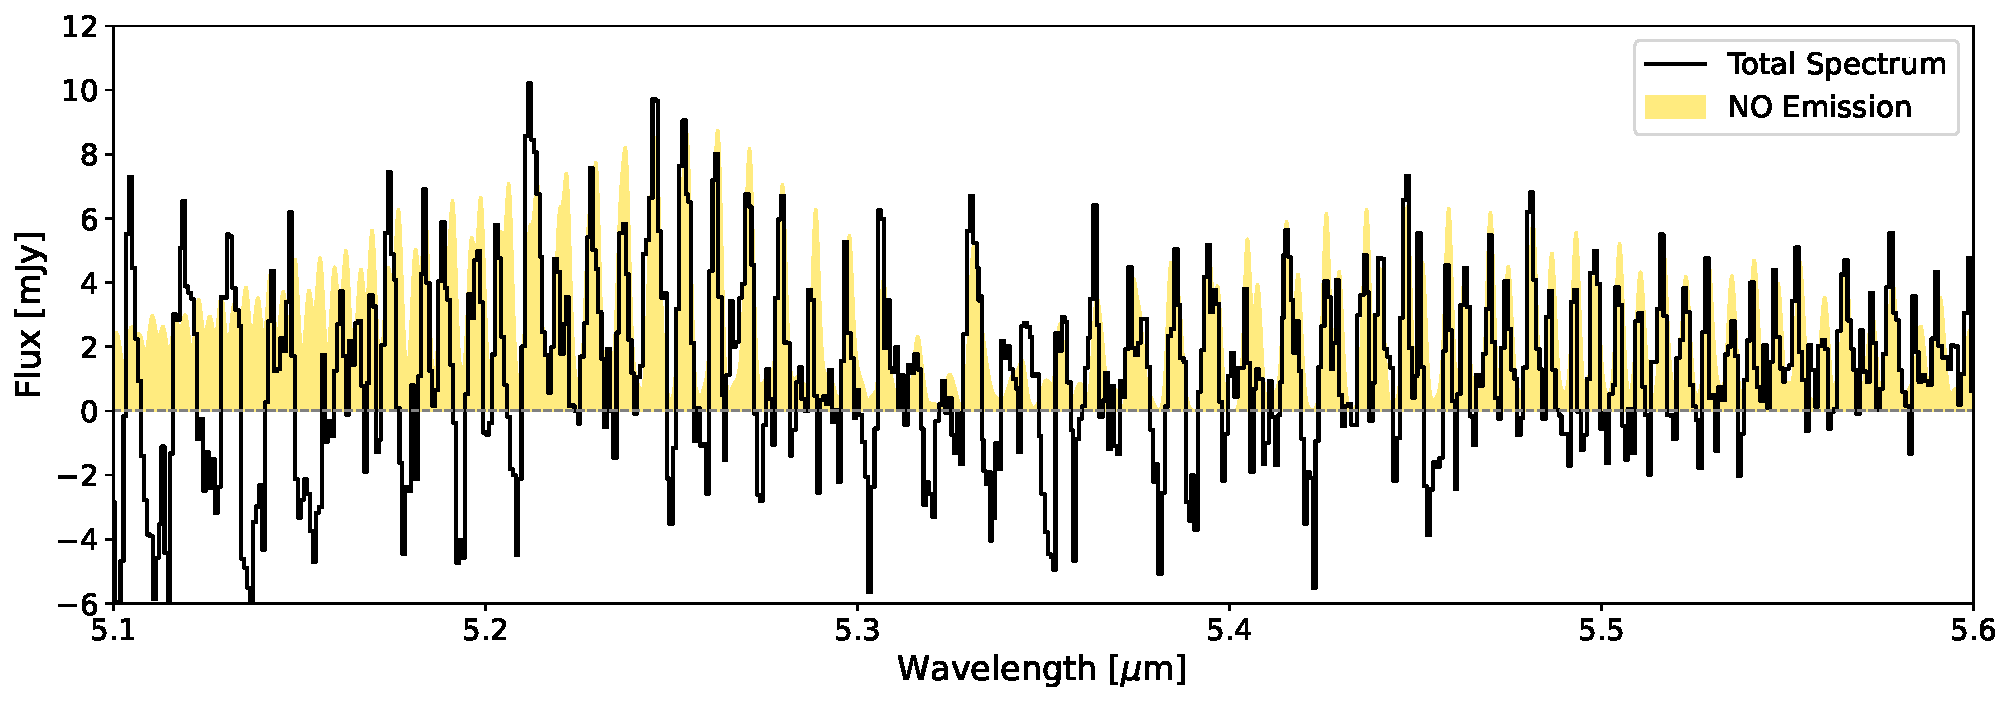
\includegraphics[width=\linewidth]{Figures/H2O_CO_removed.pdf}
    \caption{A zoomed-in region of the spectrum of the fiducial model between 4.9 $\mu$m and 6 $\mu$m. The emission of both H\2O and CO has been removed.}
    \label{fig: H2O and CO removed}
\end{figure}

\section{Application of Detection Methods to JWST Observations}
After the confirmation that this technique is valid on the simulated spectra, we applied it to real data to see if they are effective here as well.

\subsection{Molecule Detection}
Using the templates generated from the emission of the species for all the ProDiMo models in the grid, we cross-correlated the templates with the measured spectra. The results of this are shown in \autoref{tab: realdata}.

\begin{table}[!ht]
\centering
\begin{tabular}{|l|ccc|}
\hline
\textbf{Molecule} & \textbf{GWLup} & \textbf{Sz98} & \textbf{V1094Sco} \\ \hline
C2H2            & Detection      & Non-detection & Detection         \\
CH4             & Non-detection  & Non-detection & Non-detection     \\
CO              & Detection      & Detection     & Detection         \\
CO2             & Detection      & Detection     & Detection         \\
H2O             & Detection      & Detection     & Detection         \\
HCN             & Detection      & Detection     & Detection         \\
NH3             & Non-detection  & Non-detection & Non-detection     \\
NO              & Non-detection  & Non-detection & Non-detection     \\
OH              & Detection      & Detection     & Detection         \\ \hline
\end{tabular}

\caption{The detection of different molecules in the spectra of GWLup, Sz98, and V1094Sco using cross-correlation.}
\label{tab: realdata}
\end{table}


LTE models were then used to fit CO and H\2O in the region 4.9-6.5 $\mu$m to the measured spectra. The resulting fits are shown in \autoref{fig: fits}.

% \begin{figure}[H]
%     \centering
%     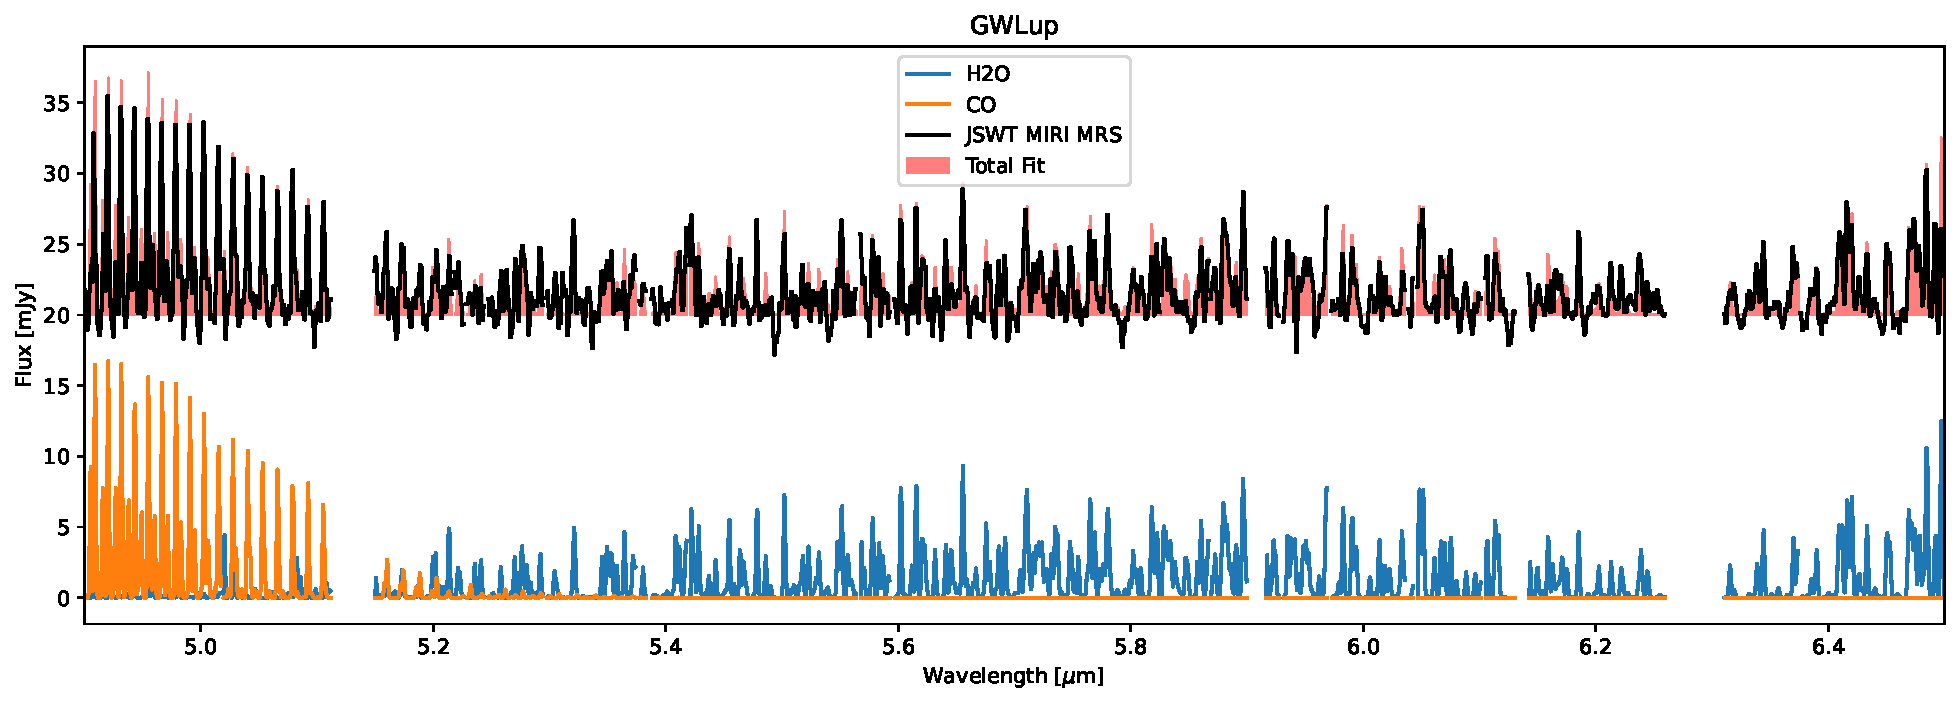
\includegraphics[width=\linewidth]{Figures/Fit_GWLup.pdf}
%     \caption{The fitted H\2O and CO spectra using a 1D LTE model between 4.9 $\mu$m and 6.5$\mu$m for GWLup}
%     \label{fig: fit gwlup}
% \end{figure}
% \begin{figure}[H]
%     \centering
%     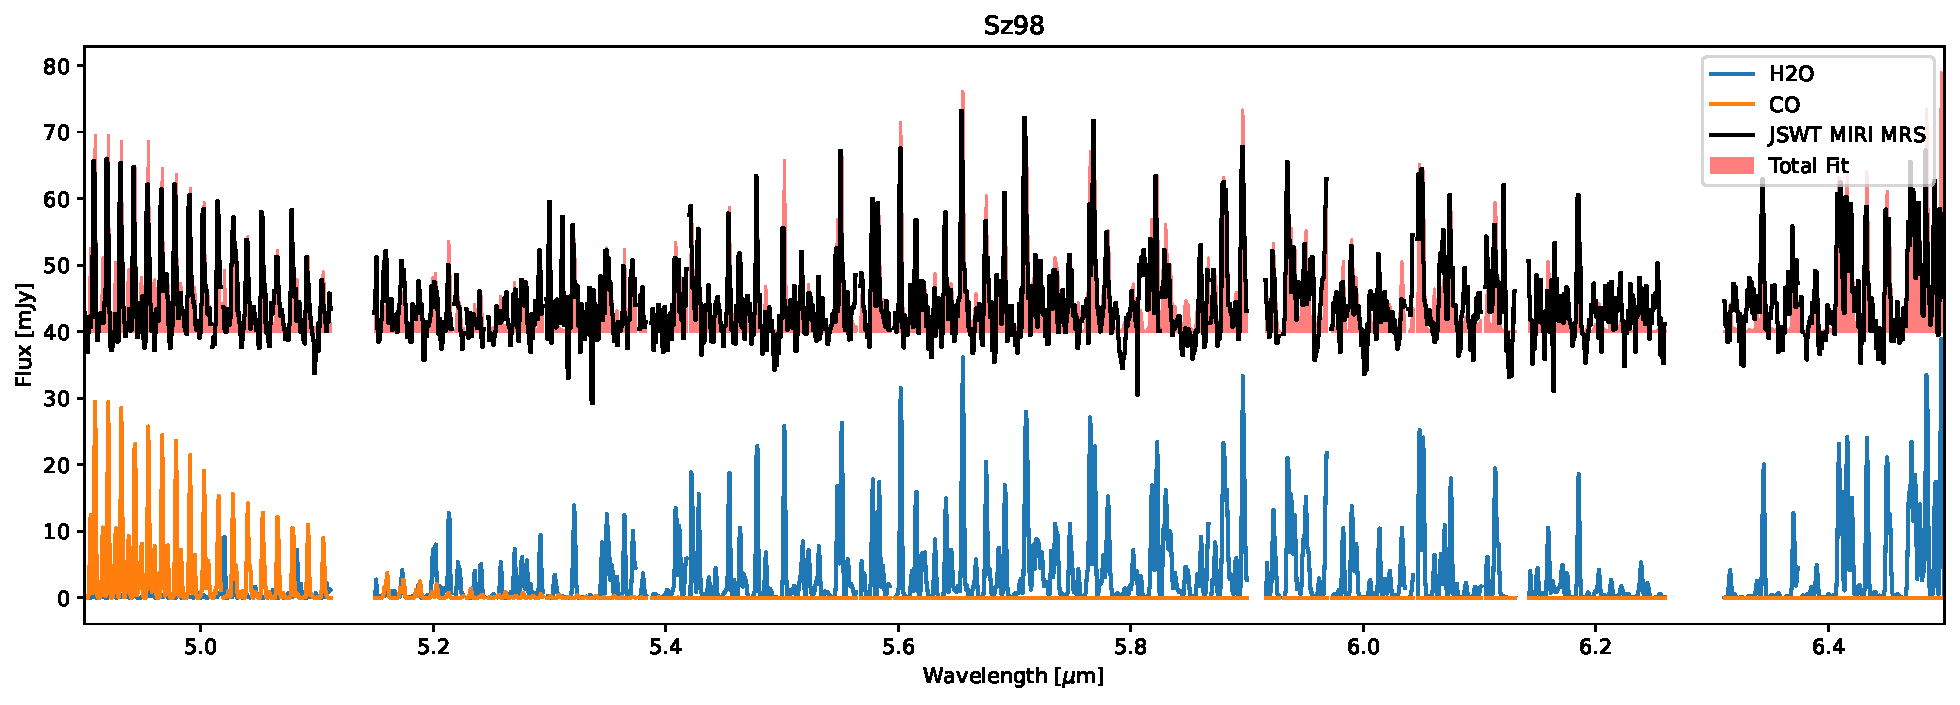
\includegraphics[width=\linewidth]{Figures/Fit_Sz98.pdf}
%     \caption{The fitted H\2O and CO spectra using a 1D LTE model between 4.9 $\mu$m and 6.5$\mu$m for Sz98}
%     \label{fig: fit sz98}
% \end{figure}
% \begin{figure}[H]
%     \centering
%     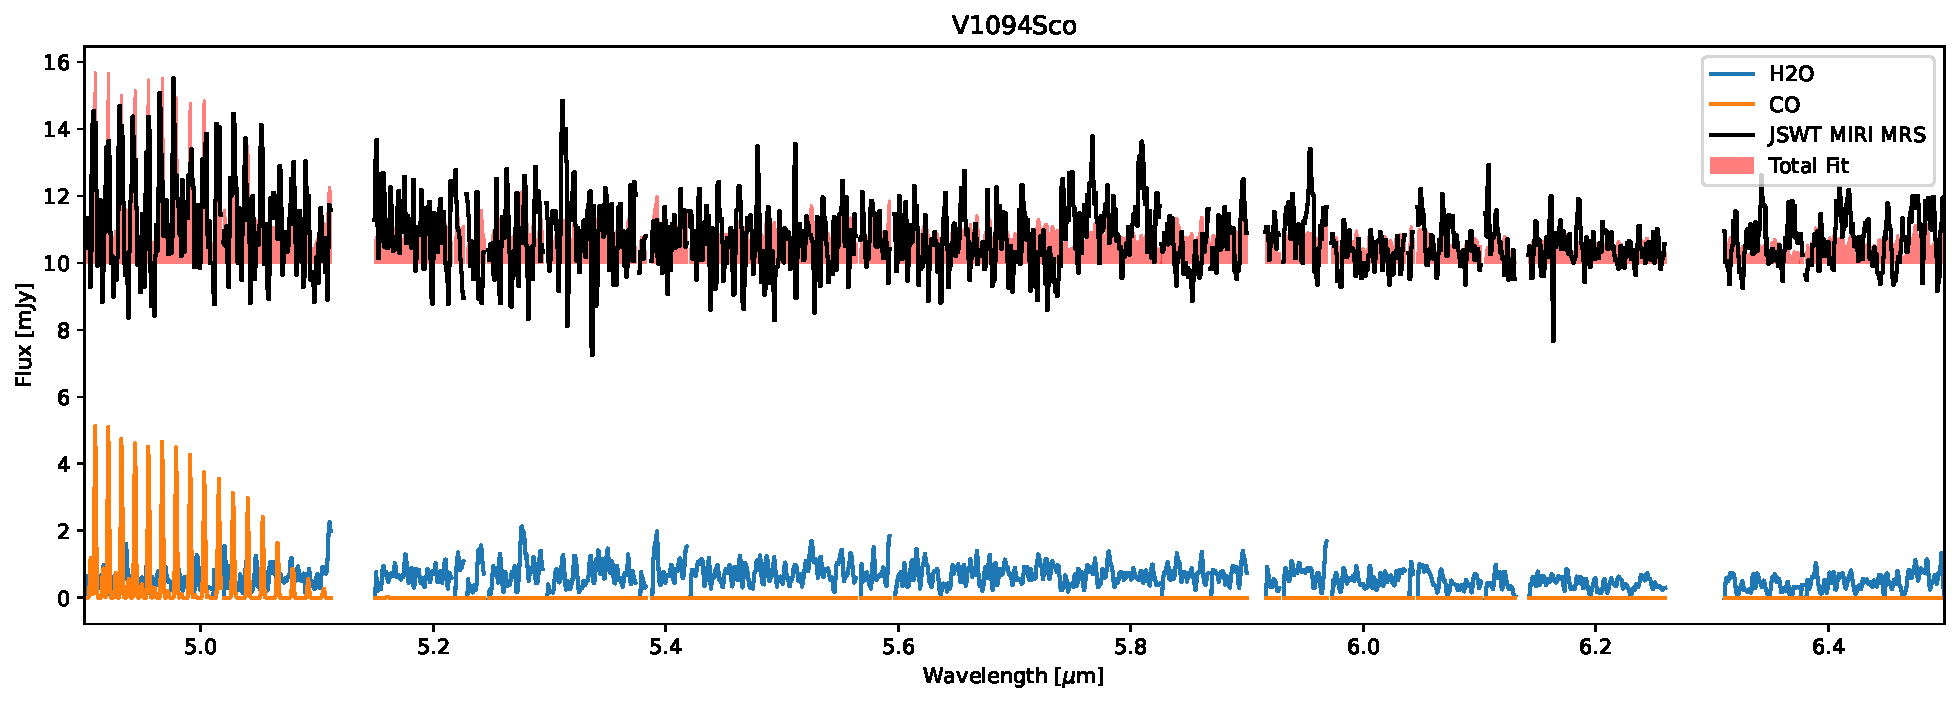
\includegraphics[width=\linewidth]{Figures/Fit_V1094Sco.pdf}
%     \caption{The fitted H\2O and CO spectra using a 1D LTE model between 4.9 $\mu$m and 6.5$\mu$m for V1094Sco}
%     \label{fig: v1094sco}
% \end{figure}
\begin{figure}[H]
    \centering
    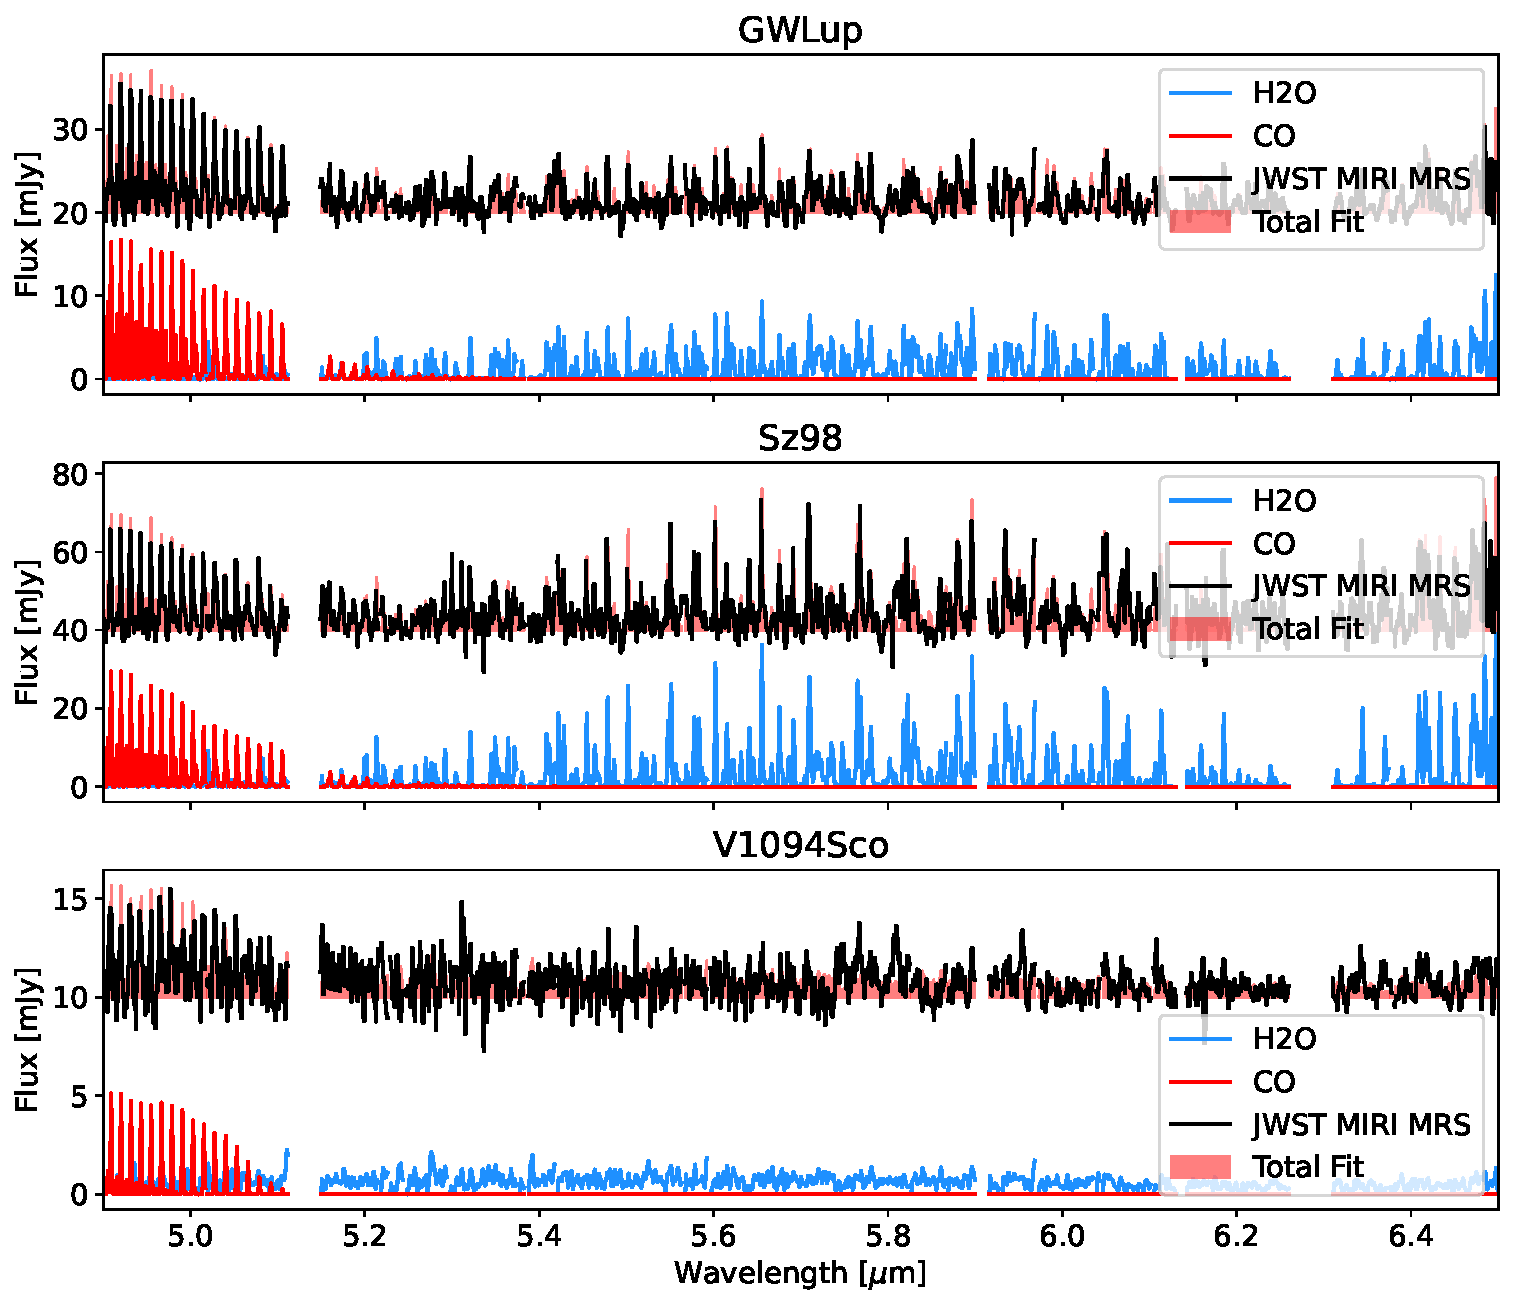
\includegraphics[width=\linewidth]{Figures/Fits.pdf}
    \caption{The fitted H\2O and CO spectra using a 0D LTE model between 4.9 $\mu$m and 6.5$\mu$m for GWLup, Sz98, and V1094Sco}
    \label{fig: fits}
\end{figure}

The fitted CO and H\2O emission was subsequently removed, and the cross-correlation technique was applied to the residuals of the spectrum. In GWLup and Sz98, no NO was detected. However, V1094Sco has a detection of NO. The residuals of V1094Sco and the scaled NO template are shown in \autoref{fig: no detect}. 
\begin{figure}[H]
    \centering
    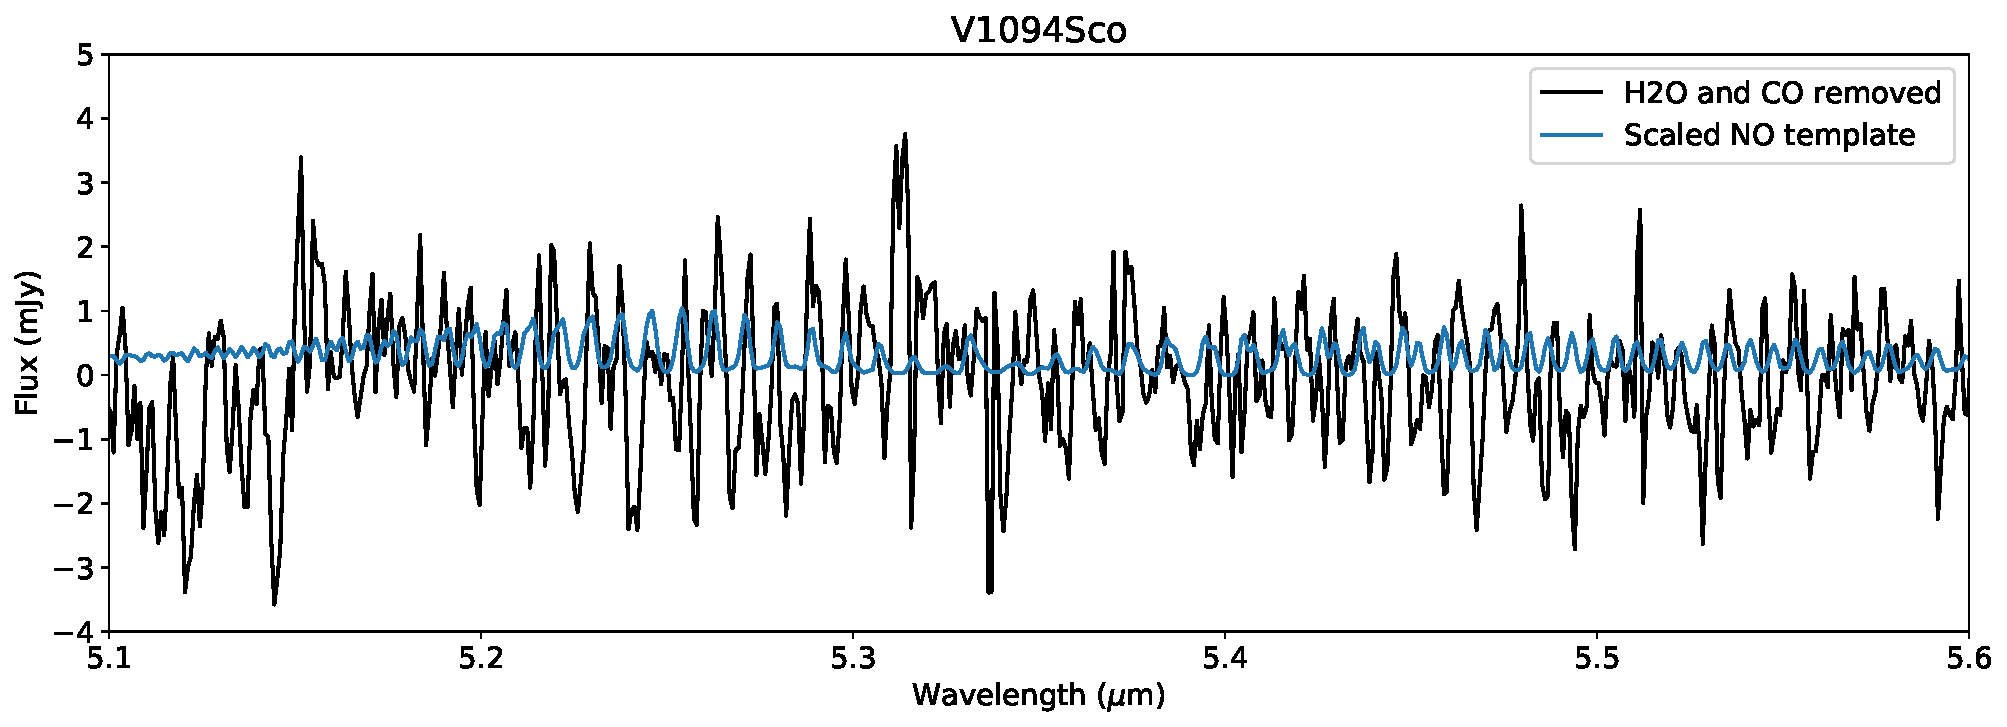
\includegraphics[width=\linewidth]{Figures/NO_Detect.pdf}
    \caption{The fitted H\2O and CO spectra using a 0D LTE model between 4.9 $\mu$m and 6.5$\mu$m for V1094Sco}
    \label{fig: no detect}
\end{figure}


\subsection{Upperlimits on NH3 and NO}

\chapter{Discussion}\label{Ch: Discussion}
\section{Interpretation}
This thesis provides new insights into the detection of nitrogen carriers NO and NH\3 in the planet-forming regions of protoplanetary disks. The influence of C and O abundances on the spectra was analyzed, which gave interesting results. The spectra formed 2 groups: spectra dominated by H\2O emission for the models that had a C/O ratio smaller than unity, and spectra dominated by C\2H\2 emission for models with C/O greater than unity. Following this, emission of both NO and NH\3 was less obscured by water lines in the spectra of the carbon-rich models, which leads to the conclusion that carbon-rich sources are the most prominent sources for the detection of NO and NH\3 in the planet-forming regions of protoplanetary disks. 

However, a direct NO and NH\3 detection from the spectrum poses to be hard due to the low intensity of the emission of these molecules and the level of noise. To combat this, we have developed a method using cross-correlation to detect weak spectral features. Using this technique on the simulated spectra generated using FLiTs gave the expected results. The most prominent features were detected in the spectrum, but not the weak emission from NO and NH\3. NO was detected in the spectrum of \textbf{WHICH MODELS} after removing the emission of CO and H\2O. However, \textbf{RESULTS ON THE REMOVAL OF ALL EMISSIONS EXCEPT NH3}


\section{Comparison to Other Works}
\cite{Grant_2023} have detected CO, CO\2, H\2O, HCN, C\2H\2 and OH in the spectrum of GWLup. These are the same molecules we detected using our cross-technique. In the spectrum of Sz98 \cite{Gasman_2023}, they have detected CO, H\2O, OH, CO\2, and HCN. These are again the same molecules we detected. The fact that we have the same results as they is a promising sign for the validity of our technique. 

\cite{groningenthesis} performed research similar to our own. However, they investigated the detection of SO\2 to learn more about the sulfur depletion problem. \textbf{MORE TEXT COMPARING OUR RESULTS}

\section{Limitations}
For the cross-correlation technique, we assume that the peak at lag=0 is purely from the molecule that is being tested. However, it could be the case that the cross-correlation of the noise with the template results in a peak, because the noise coincidentally follows a similar structure to the emission of the species. We suspect that this is highly unlikely, as the noise would then need to be in the same location (i.e., not shifted to different wavelengths) and follow a similar pattern (i.e., be bright in the same locations as the molecular emission). A problem that might be more impactful is fringing. Fringing is the effect when taking a spectrum that results in a regular pattern. This pattern could coincide with the pattern formed by the ro-vibrational transitions, which also has a regular spacing. If it were the case that these two phenomena would overlap, that could result in a false-positive.

Other than noise, other species could also interfere with our method of cross-correlation. When the emission of different spectra overlaps, that could result in a detection. For example, in \autoref{fig: NO region} the CO emission partly overlaps with the emission coming from NO. This, with the fact that the spacing of the two species is similar, could result in false positives. 

Following this, we use bootstrapping to create the hypothesis test by sampling the distribution of the test statistic. However, this destroys all patterns in the data. This can give a disproportionate view of the significance of a species' presence, leading to a false-positive.

Averaging the emission of all species across the entire grid may not be the best technique for creating a template. The different abundances heavily impact the shape of the emission and combining them into a single template results the a spectrum that has about the same shape, but can lose.

\section{Future Work}
In this work, the only things that were varied were the C and O abundances. Some other properties could be interesting to investigate, for example, different disk structures. The distribution of NH\3 in \autoref{fig: nitrogen distribution}, is close to the midplane in the disk, resulting in it being hidden inside the disk. Different disk structures, such as gaps, could expose the NH\3 reservoir, allowing for detection. 

Furthermore, the stellar properties could affect the nitrogen carriers in the disk. Changing attributes such as stellar luminosity, mass, and temperature can result in different chemistries in the disk, thereby altering the spectrum that is measured. 

Improving models to account for additional species or more realistic noise.

Refining spectral resolution and detection limits using advanced filters.

\chapter{Conclusion}\label{Ch: Conclusion}
In this thesis, we have looked at the influence of the carbon and oxygen abundances on the nitrogen carriers in a protoplanetary disk and applied that knowledge to JWST MIRI MRS observations. Our main conclusions are as follows:
\begin{itemize}
    \item \textbf{SOMETHING ABOUT THE EFFECT OF C AND O ON FLUX}
    \item We have selected spectral regions, in which the emission from NO and NH\3 are the strongest. In particular, sources with a C/O ratio greater than unity have the greatest potential for detecting NO and NH\3 as their emission is not obscured by H\2O emission.
    \item We developed a new molecule detection method using cross-correlation. Using the ProDiMo models in the grid, emission templates per species were created. 
    \item We reconfirmed the known species present in the spectra of GWLup, Sz98, and V1094Sco using the cross-correlation technique.
    \item We made a possible detection of NO in the spectrum of V1094Sco.
    \item \textbf{UPPERLIMITS ON THE SOURCES}
\end{itemize}

\bibliographystyle{aa.bst}
\bibliography{references}
\appendix
\chapter{More ProDiMo Results}
\chapter{Chi square fits}
\end{document}